\documentclass[1p]{elsarticle_modified}
%\bibliographystyle{elsarticle-num}

%\usepackage[colorlinks]{hyperref}
%\usepackage{abbrmath_seonhwa} %\Abb, \Ascr, \Acal ,\Abf, \Afrak
\usepackage{amsfonts}
\usepackage{amssymb}
\usepackage{amsmath}
\usepackage{amsthm}
\usepackage{scalefnt}
\usepackage{amsbsy}
\usepackage{kotex}
\usepackage{caption}
\usepackage{subfig}
\usepackage{color}
\usepackage{graphicx}
\usepackage{xcolor} %% white, black, red, green, blue, cyan, magenta, yellow
\usepackage{float}
\usepackage{setspace}
\usepackage{hyperref}

\usepackage{tikz}
\usetikzlibrary{arrows}

\usepackage{multirow}
\usepackage{array} % fixed length table
\usepackage{hhline}

%%%%%%%%%%%%%%%%%%%%%
\makeatletter
\renewcommand*\env@matrix[1][\arraystretch]{%
	\edef\arraystretch{#1}%
	\hskip -\arraycolsep
	\let\@ifnextchar\new@ifnextchar
	\array{*\c@MaxMatrixCols c}}
\makeatother %https://tex.stackexchange.com/questions/14071/how-can-i-increase-the-line-spacing-in-a-matrix
%%%%%%%%%%%%%%%

\usepackage[normalem]{ulem}

\newcommand{\msout}[1]{\ifmmode\text{\sout{\ensuremath{#1}}}\else\sout{#1}\fi}
%SOURCE: \msout is \stkout macro in https://tex.stackexchange.com/questions/20609/strikeout-in-math-mode

\newcommand{\cancel}[1]{
	\ifmmode
	{\color{red}\msout{#1}}
	\else
	{\color{red}\sout{#1}}
	\fi
}

\newcommand{\add}[1]{
	{\color{blue}\uwave{#1}}
}

\newcommand{\replace}[2]{
	\ifmmode
	{\color{red}\msout{#1}}{\color{blue}\uwave{#2}}
	\else
	{\color{red}\sout{#1}}{\color{blue}\uwave{#2}}
	\fi
}

\newcommand{\Sol}{\mathcal{S}} %segment
\newcommand{\D}{D} %diagram
\newcommand{\A}{\mathcal{A}} %arc


%%%%%%%%%%%%%%%%%%%%%%%%%%%%%5 test

\def\sl{\operatorname{\textup{SL}}(2,\Cbb)}
\def\psl{\operatorname{\textup{PSL}}(2,\Cbb)}
\def\quan{\mkern 1mu \triangleright \mkern 1mu}

\theoremstyle{definition}
\newtheorem{thm}{Theorem}[section]
\newtheorem{prop}[thm]{Proposition}
\newtheorem{lem}[thm]{Lemma}
\newtheorem{ques}[thm]{Question}
\newtheorem{cor}[thm]{Corollary}
\newtheorem{defn}[thm]{Definition}
\newtheorem{exam}[thm]{Example}
\newtheorem{rmk}[thm]{Remark}
\newtheorem{alg}[thm]{Algorithm}

\newcommand{\I}{\sqrt{-1}}
\begin{document}

%\begin{frontmatter}
%
%\title{Boundary parabolic representations of knots up to 8 crossings}
%
%%% Group authors per affiliation:
%\author{Yunhi Cho} 
%\address{Department of Mathematics, University of Seoul, Seoul, Korea}
%\ead{yhcho@uos.ac.kr}
%
%
%\author{Seonhwa Kim} %\fnref{s_kim}}
%\address{Center for Geometry and Physics, Institute for Basic Science, Pohang, 37673, Korea}
%\ead{ryeona17@ibs.re.kr}
%
%\author{Hyuk Kim}
%\address{Department of Mathematical Sciences, Seoul National University, Seoul 08826, Korea}
%\ead{hyukkim@snu.ac.kr}
%
%\author{Seokbeom Yoon}
%\address{Department of Mathematical Sciences, Seoul National University, Seoul, 08826,  Korea}
%\ead{sbyoon15@snu.ac.kr}
%
%\begin{abstract}
%We find all boundary parabolic representation of knots up to 8 crossings.
%
%\end{abstract}
%\begin{keyword}
%    \MSC[2010] 57M25 
%\end{keyword}
%
%\end{frontmatter}

%\linenumbers
%\tableofcontents
%
\newcommand\colored[1]{\textcolor{white}{\rule[-0.35ex]{0.8em}{1.4ex}}\kern-0.8em\color{red} #1}%
%\newcommand\colored[1]{\textcolor{white}{ #1}\kern-2.17ex	\textcolor{white}{ #1}\kern-1.81ex	\textcolor{white}{ #1}\kern-2.15ex\color{red}#1	}

{\Large $\underline{12a_{0965}~(K12a_{0965})}$}

\setlength{\tabcolsep}{10pt}
\renewcommand{\arraystretch}{1.6}
\vspace{1cm}\begin{tabular}{m{100pt}>{\centering\arraybackslash}m{274pt}}
\multirow{5}{120pt}{
	\centering
	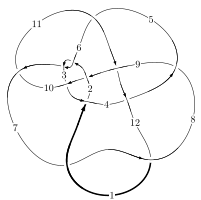
\includegraphics[width=112pt]{../../../GIT/diagram.site/Diagrams/png/1766_12a_0965.png}\\
\ \ \ A knot diagram\footnotemark}&
\allowdisplaybreaks
\textbf{Linearized knot diagam} \\
\cline{2-2}
 &
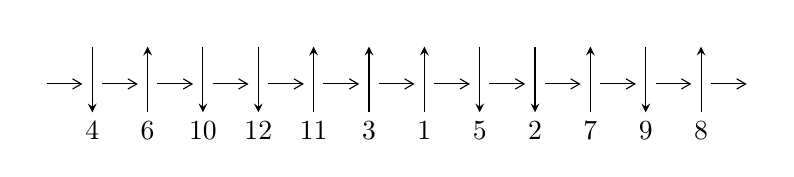
\begin{tikzpicture}[x=20pt, y=17pt]
	% nodes
	\node (C0) at (0, 0) {};
	\node (C1) at (1, 0) {};
	\node (C1U) at (1, +1) {};
	\node (C1D) at (1, -1) {4};

	\node (C2) at (2, 0) {};
	\node (C2U) at (2, +1) {};
	\node (C2D) at (2, -1) {6};

	\node (C3) at (3, 0) {};
	\node (C3U) at (3, +1) {};
	\node (C3D) at (3, -1) {10};

	\node (C4) at (4, 0) {};
	\node (C4U) at (4, +1) {};
	\node (C4D) at (4, -1) {12};

	\node (C5) at (5, 0) {};
	\node (C5U) at (5, +1) {};
	\node (C5D) at (5, -1) {11};

	\node (C6) at (6, 0) {};
	\node (C6U) at (6, +1) {};
	\node (C6D) at (6, -1) {3};

	\node (C7) at (7, 0) {};
	\node (C7U) at (7, +1) {};
	\node (C7D) at (7, -1) {1};

	\node (C8) at (8, 0) {};
	\node (C8U) at (8, +1) {};
	\node (C8D) at (8, -1) {5};

	\node (C9) at (9, 0) {};
	\node (C9U) at (9, +1) {};
	\node (C9D) at (9, -1) {2};

	\node (C10) at (10, 0) {};
	\node (C10U) at (10, +1) {};
	\node (C10D) at (10, -1) {7};

	\node (C11) at (11, 0) {};
	\node (C11U) at (11, +1) {};
	\node (C11D) at (11, -1) {9};

	\node (C12) at (12, 0) {};
	\node (C12U) at (12, +1) {};
	\node (C12D) at (12, -1) {8};
	\node (C13) at (13, 0) {};

	% arrows
	\draw[->,>={angle 60}]
	(C0) edge (C1) (C1) edge (C2) (C2) edge (C3) (C3) edge (C4) (C4) edge (C5) (C5) edge (C6) (C6) edge (C7) (C7) edge (C8) (C8) edge (C9) (C9) edge (C10) (C10) edge (C11) (C11) edge (C12) (C12) edge (C13) ;	\draw[->,>=stealth]
	(C1U) edge (C1D) (C2D) edge (C2U) (C3U) edge (C3D) (C4U) edge (C4D) (C5D) edge (C5U) (C6D) edge (C6U) (C7D) edge (C7U) (C8U) edge (C8D) (C9U) edge (C9D) (C10D) edge (C10U) (C11U) edge (C11D) (C12D) edge (C12U) ;
	\end{tikzpicture} \\
\hhline{~~} \\& 
\textbf{Solving Sequence} \\ \cline{2-2} 
 &
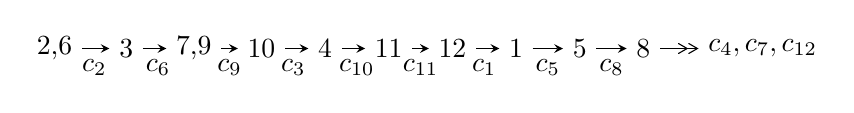
\begin{tikzpicture}[x=23pt, y=7pt]
	% node
	\node (A0) at (-1/8, 0) {2,6};
	\node (A1) at (1, 0) {3};
	\node (A2) at (33/16, 0) {7,9};
	\node (A3) at (25/8, 0) {10};
	\node (A4) at (33/8, 0) {4};
	\node (A5) at (41/8, 0) {11};
	\node (A6) at (49/8, 0) {12};
	\node (A7) at (57/8, 0) {1};
	\node (A8) at (65/8, 0) {5};
	\node (A9) at (73/8, 0) {8};
	\node (C1) at (1/2, -1) {$c_{2}$};
	\node (C2) at (3/2, -1) {$c_{6}$};
	\node (C3) at (21/8, -1) {$c_{9}$};
	\node (C4) at (29/8, -1) {$c_{3}$};
	\node (C5) at (37/8, -1) {$c_{10}$};
	\node (C6) at (45/8, -1) {$c_{11}$};
	\node (C7) at (53/8, -1) {$c_{1}$};
	\node (C8) at (61/8, -1) {$c_{5}$};
	\node (C9) at (69/8, -1) {$c_{8}$};
	\node (A10) at (11, 0) {$c_{4},c_{7},c_{12}$};

	% edge
	\draw[->,>=stealth]	
	(A0) edge (A1) (A1) edge (A2) (A2) edge (A3) (A3) edge (A4) (A4) edge (A5) (A5) edge (A6) (A6) edge (A7) (A7) edge (A8) (A8) edge (A9) ;
	\draw[->>,>={angle 60}]	
	(A9) edge (A10);
\end{tikzpicture} \\ 

\end{tabular} \\

\footnotetext{
The image of knot diagram is generated by the software ``\textbf{Draw programme}" developed by Andrew Bartholomew(\url{http://www.layer8.co.uk/maths/draw/index.htm\#Running-draw}), where we modified some parts for our purpose(\url{https://github.com/CATsTAILs/LinksPainter}).
}\phantom \\ \newline 
\centering \textbf{Ideals for irreducible components\footnotemark of $X_{\text{par}}$} 
 
\begin{align*}
I^u_{1}&=\langle 
5.70198\times10^{1113} u^{193}-5.06279\times10^{1113} u^{192}+\cdots+2.49058\times10^{1112} b+3.40214\times10^{1117},\\
\phantom{I^u_{1}}&\phantom{= \langle  }7.87713\times10^{1117} u^{193}-6.57773\times10^{1117} u^{192}+\cdots+1.33271\times10^{1116} a+5.04524\times10^{1121},\\
\phantom{I^u_{1}}&\phantom{= \langle  }u^{194}-58 u^{192}+\cdots-41332 u+5351\rangle \\
I^u_{2}&=\langle 
-1.13596\times10^{59} u^{45}+6.86725\times10^{58} u^{44}+\cdots+1.72718\times10^{58} b+2.87571\times10^{60},\\
\phantom{I^u_{2}}&\phantom{= \langle  }-8.87801\times10^{60} u^{45}+1.72576\times10^{61} u^{44}+\cdots+6.39057\times10^{59} a-4.86320\times10^{62},\\
\phantom{I^u_{2}}&\phantom{= \langle  }u^{46}- u^{45}+\cdots-52 u+37\rangle \\
\\
\end{align*}
\raggedright * 2 irreducible components of $\dim_{\mathbb{C}}=0$, with total 240 representations.\\
\footnotetext{All coefficients of polynomials are rational numbers. But the coefficients are sometimes approximated in decimal forms when there is not enough margin.}
\newpage
\renewcommand{\arraystretch}{1}
\centering \section*{I. $I^u_{1}= \langle 5.70\times10^{1113} u^{193}-5.06\times10^{1113} u^{192}+\cdots+2.49\times10^{1112} b+3.40\times10^{1117},\;7.88\times10^{1117} u^{193}-6.58\times10^{1117} u^{192}+\cdots+1.33\times10^{1116} a+5.05\times10^{1121},\;u^{194}-58 u^{192}+\cdots-41332 u+5351 \rangle$}
\flushleft \textbf{(i) Arc colorings}\\
\begin{tabular}{m{7pt} m{180pt} m{7pt} m{180pt} }
\flushright $a_{2}=$&$\begin{pmatrix}1\\0\end{pmatrix}$ \\
\flushright $a_{6}=$&$\begin{pmatrix}0\\u\end{pmatrix}$ \\
\flushright $a_{3}=$&$\begin{pmatrix}1\\- u^2\end{pmatrix}$ \\
\flushright $a_{7}=$&$\begin{pmatrix}u\\- u^3+u\end{pmatrix}$ \\
\flushright $a_{9}=$&$\begin{pmatrix}-59.1062 u^{193}+49.3561 u^{192}+\cdots+3.37605\times10^{6} u-378571.\\-22.8942 u^{193}+20.3278 u^{192}+\cdots+1.20662\times10^{6} u-136601.\end{pmatrix}$ \\
\flushright $a_{10}=$&$\begin{pmatrix}-36.2119 u^{193}+29.0283 u^{192}+\cdots+2.16943\times10^{6} u-241970.\\-22.8942 u^{193}+20.3278 u^{192}+\cdots+1.20662\times10^{6} u-136601.\end{pmatrix}$ \\
\flushright $a_{4}=$&$\begin{pmatrix}462.081 u^{193}-402.665 u^{192}+\cdots-2.50795\times10^{7} u+2.82883\times10^{6}\\112.319 u^{193}-101.833 u^{192}+\cdots-5.83845\times10^{6} u+661585.\end{pmatrix}$ \\
\flushright $a_{11}=$&$\begin{pmatrix}-45.4132 u^{193}+37.5799 u^{192}+\cdots+2.60857\times10^{6} u-292161.\\-23.9760 u^{193}+21.4281 u^{192}+\cdots+1.24308\times10^{6} u-141033.\end{pmatrix}$ \\
\flushright $a_{12}=$&$\begin{pmatrix}37.1151 u^{193}-37.1502 u^{192}+\cdots-1.72919\times10^{6} u+198801.\\4.35805 u^{193}-4.25435 u^{192}+\cdots-223358. u+25314.2\end{pmatrix}$ \\
\flushright $a_{1}=$&$\begin{pmatrix}-1906.95 u^{193}+1772.17 u^{192}+\cdots+9.65016\times10^{7} u-1.09687\times10^{7}\\-293.512 u^{193}+275.886 u^{192}+\cdots+1.46532\times10^{7} u-1.66814\times10^{6}\end{pmatrix}$ \\
\flushright $a_{5}=$&$\begin{pmatrix}411.748 u^{193}-359.640 u^{192}+\cdots-2.23091\times10^{7} u+2.51690\times10^{6}\\99.5315 u^{193}-90.3895 u^{192}+\cdots-5.16861\times10^{6} u+585822.\end{pmatrix}$ \\
\flushright $a_{8}=$&$\begin{pmatrix}-1576.82 u^{193}+1386.91 u^{192}+\cdots+8.48206\times10^{7} u-9.57661\times10^{6}\\-363.820 u^{193}+324.005 u^{192}+\cdots+1.93187\times10^{7} u-2.18417\times10^{6}\end{pmatrix}$\\&\end{tabular}
\flushleft \textbf{(ii) Obstruction class $= -1$}\\~\\
\flushleft \textbf{(iii) Cusp Shapes $= 1479.28 u^{193}-1327.25 u^{192}+\cdots-7.80477\times10^{7} u+8.82846\times10^{6}$}\\~\\
\newpage\renewcommand{\arraystretch}{1}
\flushleft \textbf{(iv) u-Polynomials at the component}\newline \\
\begin{tabular}{m{50pt}|m{274pt}}
Crossings & \hspace{64pt}u-Polynomials at each crossing \\
\hline $$\begin{aligned}c_{1}\end{aligned}$$&$\begin{aligned}
&u^{194}-14 u^{193}+\cdots-10335075 u+452173
\end{aligned}$\\
\hline $$\begin{aligned}c_{2},c_{6}\end{aligned}$$&$\begin{aligned}
&u^{194}-58 u^{192}+\cdots+41332 u+5351
\end{aligned}$\\
\hline $$\begin{aligned}c_{3}\end{aligned}$$&$\begin{aligned}
&u^{194}-7 u^{193}+\cdots+39248422 u+9682667
\end{aligned}$\\
\hline $$\begin{aligned}c_{4}\end{aligned}$$&$\begin{aligned}
&u^{194}-10 u^{192}+\cdots+592 u+32
\end{aligned}$\\
\hline $$\begin{aligned}c_{5}\end{aligned}$$&$\begin{aligned}
&u^{194}-7 u^{193}+\cdots+8037239426 u+414181957
\end{aligned}$\\
\hline $$\begin{aligned}c_{7},c_{12}\end{aligned}$$&$\begin{aligned}
&u^{194}+73 u^{192}+\cdots+2028865 u+69361
\end{aligned}$\\
\hline $$\begin{aligned}c_{8}\end{aligned}$$&$\begin{aligned}
&u^{194}-5 u^{193}+\cdots+20845830 u+2067743
\end{aligned}$\\
\hline $$\begin{aligned}c_{9}\end{aligned}$$&$\begin{aligned}
&u^{194}+25 u^{192}+\cdots-128757 u+4502
\end{aligned}$\\
\hline $$\begin{aligned}c_{10}\end{aligned}$$&$\begin{aligned}
&u^{194}-3 u^{192}+\cdots+58245120 u+4562944
\end{aligned}$\\
\hline $$\begin{aligned}c_{11}\end{aligned}$$&$\begin{aligned}
&u^{194}+7 u^{193}+\cdots-1621 u+64
\end{aligned}$\\
\hline
\end{tabular}\\~\\
\newpage\renewcommand{\arraystretch}{1}
\flushleft \textbf{(v) Riley Polynomials at the component}\newline \\
\begin{tabular}{m{50pt}|m{274pt}}
Crossings & \hspace{64pt}Riley Polynomials at each crossing \\
\hline $$\begin{aligned}c_{1}\end{aligned}$$&$\begin{aligned}
&y^{194}+30 y^{193}+\cdots+24812515342591 y+204460421929
\end{aligned}$\\
\hline $$\begin{aligned}c_{2},c_{6}\end{aligned}$$&$\begin{aligned}
&y^{194}-116 y^{193}+\cdots-698910882 y+28633201
\end{aligned}$\\
\hline $$\begin{aligned}c_{3}\end{aligned}$$&$\begin{aligned}
&y^{194}+33 y^{193}+\cdots+6027177013969630 y+93754040232889
\end{aligned}$\\
\hline $$\begin{aligned}c_{4}\end{aligned}$$&$\begin{aligned}
&y^{194}-20 y^{193}+\cdots-3328 y+1024
\end{aligned}$\\
\hline $$\begin{aligned}c_{5}\end{aligned}$$&$\begin{aligned}
&y^{194}+43 y^{193}+\cdots+1.01\times10^{19} y+1.72\times10^{17}
\end{aligned}$\\
\hline $$\begin{aligned}c_{7},c_{12}\end{aligned}$$&$\begin{aligned}
&y^{194}+146 y^{193}+\cdots+47660025157 y+4810948321
\end{aligned}$\\
\hline $$\begin{aligned}c_{8}\end{aligned}$$&$\begin{aligned}
&y^{194}-59 y^{193}+\cdots-302813164355902 y+4275561114049
\end{aligned}$\\
\hline $$\begin{aligned}c_{9}\end{aligned}$$&$\begin{aligned}
&y^{194}+50 y^{193}+\cdots-2034708073 y+20268004
\end{aligned}$\\
\hline $$\begin{aligned}c_{10}\end{aligned}$$&$\begin{aligned}
&y^{194}-6 y^{193}+\cdots-1452285242638336 y+20820457947136
\end{aligned}$\\
\hline $$\begin{aligned}c_{11}\end{aligned}$$&$\begin{aligned}
&y^{194}+17 y^{193}+\cdots+497991 y+4096
\end{aligned}$\\
\hline
\end{tabular}\\~\\
\newpage\flushleft \textbf{(vi) Complex Volumes and Cusp Shapes}
$$\begin{array}{c|c|c}  
\text{Solutions to }I^u_{1}& \I (\text{vol} + \sqrt{-1}CS) & \text{Cusp shape}\\
 \hline 
\begin{aligned}
u &= \phantom{-}0.947923 + 0.331996 I \\
a &= \phantom{-}0.572807 + 0.288540 I \\
b &= \phantom{-}1.50681 + 0.26720 I\end{aligned}
 & -2.68206 + 4.37253 I & \phantom{-0.000000 } 0 \\ \hline\begin{aligned}
u &= \phantom{-}0.947923 - 0.331996 I \\
a &= \phantom{-}0.572807 - 0.288540 I \\
b &= \phantom{-}1.50681 - 0.26720 I\end{aligned}
 & -2.68206 - 4.37253 I & \phantom{-0.000000 } 0 \\ \hline\begin{aligned}
u &= -0.981969 + 0.224704 I \\
a &= -0.891442 - 0.223944 I \\
b &= -0.958084 + 0.949547 I\end{aligned}
 & -3.13647 - 0.02983 I & \phantom{-0.000000 } 0 \\ \hline\begin{aligned}
u &= -0.981969 - 0.224704 I \\
a &= -0.891442 + 0.223944 I \\
b &= -0.958084 - 0.949547 I\end{aligned}
 & -3.13647 + 0.02983 I & \phantom{-0.000000 } 0 \\ \hline\begin{aligned}
u &= -0.978684 + 0.165722 I \\
a &= \phantom{-}1.79995 - 0.83672 I \\
b &= \phantom{-}1.141760 + 0.208392 I\end{aligned}
 & \phantom{-}0.47696 - 2.42283 I & \phantom{-0.000000 } 0 \\ \hline\begin{aligned}
u &= -0.978684 - 0.165722 I \\
a &= \phantom{-}1.79995 + 0.83672 I \\
b &= \phantom{-}1.141760 - 0.208392 I\end{aligned}
 & \phantom{-}0.47696 + 2.42283 I & \phantom{-0.000000 } 0 \\ \hline\begin{aligned}
u &= -0.971757 + 0.189617 I \\
a &= -0.71447 + 1.22597 I \\
b &= -1.37538 - 1.61085 I\end{aligned}
 & \phantom{-}2.03903 - 5.82281 I & \phantom{-0.000000 } 0 \\ \hline\begin{aligned}
u &= -0.971757 - 0.189617 I \\
a &= -0.71447 - 1.22597 I \\
b &= -1.37538 + 1.61085 I\end{aligned}
 & \phantom{-}2.03903 + 5.82281 I & \phantom{-0.000000 } 0 \\ \hline\begin{aligned}
u &= \phantom{-}0.242740 + 0.959618 I \\
a &= -0.119747 - 0.662601 I \\
b &= -0.491653 - 0.652462 I\end{aligned}
 & -6.24043 - 1.77674 I & \phantom{-0.000000 } 0 \\ \hline\begin{aligned}
u &= \phantom{-}0.242740 - 0.959618 I \\
a &= -0.119747 + 0.662601 I \\
b &= -0.491653 + 0.652462 I\end{aligned}
 & -6.24043 + 1.77674 I & \phantom{-0.000000 } 0\\
 \hline 
 \end{array}$$\newpage$$\begin{array}{c|c|c}  
\text{Solutions to }I^u_{1}& \I (\text{vol} + \sqrt{-1}CS) & \text{Cusp shape}\\
 \hline 
\begin{aligned}
u &= -0.919086 + 0.366049 I \\
a &= -1.46999 - 0.03993 I \\
b &= -0.680198 - 0.400565 I\end{aligned}
 & \phantom{-}1.62786 - 2.00278 I & \phantom{-0.000000 } 0 \\ \hline\begin{aligned}
u &= -0.919086 - 0.366049 I \\
a &= -1.46999 + 0.03993 I \\
b &= -0.680198 + 0.400565 I\end{aligned}
 & \phantom{-}1.62786 + 2.00278 I & \phantom{-0.000000 } 0 \\ \hline\begin{aligned}
u &= -1.005110 + 0.111196 I \\
a &= \phantom{-}1.97347 - 2.78647 I \\
b &= \phantom{-}0.983588 + 0.558412 I\end{aligned}
 & \phantom{-}0.04601 - 2.40068 I & \phantom{-0.000000 } 0 \\ \hline\begin{aligned}
u &= -1.005110 - 0.111196 I \\
a &= \phantom{-}1.97347 + 2.78647 I \\
b &= \phantom{-}0.983588 - 0.558412 I\end{aligned}
 & \phantom{-}0.04601 + 2.40068 I & \phantom{-0.000000 } 0 \\ \hline\begin{aligned}
u &= \phantom{-}1.019800 + 0.016340 I \\
a &= \phantom{-}0.867013 + 0.710888 I \\
b &= \phantom{-}1.83714 - 0.41899 I\end{aligned}
 & \phantom{-}0.85840 - 5.37053 I & \phantom{-0.000000 } 0 \\ \hline\begin{aligned}
u &= \phantom{-}1.019800 - 0.016340 I \\
a &= \phantom{-}0.867013 - 0.710888 I \\
b &= \phantom{-}1.83714 + 0.41899 I\end{aligned}
 & \phantom{-}0.85840 + 5.37053 I & \phantom{-0.000000 } 0 \\ \hline\begin{aligned}
u &= -0.416479 + 0.935043 I \\
a &= \phantom{-}0.394206 + 0.046646 I \\
b &= \phantom{-}0.665562 + 0.328631 I\end{aligned}
 & -1.45555 - 7.40018 I & \phantom{-0.000000 } 0 \\ \hline\begin{aligned}
u &= -0.416479 - 0.935043 I \\
a &= \phantom{-}0.394206 - 0.046646 I \\
b &= \phantom{-}0.665562 - 0.328631 I\end{aligned}
 & -1.45555 + 7.40018 I & \phantom{-0.000000 } 0 \\ \hline\begin{aligned}
u &= -0.299064 + 0.919963 I \\
a &= \phantom{-}1.26393 - 0.72352 I \\
b &= \phantom{-}1.002330 - 0.798991 I\end{aligned}
 & -4.64751 + 7.03213 I & \phantom{-0.000000 } 0 \\ \hline\begin{aligned}
u &= -0.299064 - 0.919963 I \\
a &= \phantom{-}1.26393 + 0.72352 I \\
b &= \phantom{-}1.002330 + 0.798991 I\end{aligned}
 & -4.64751 - 7.03213 I & \phantom{-0.000000 } 0\\
 \hline 
 \end{array}$$\newpage$$\begin{array}{c|c|c}  
\text{Solutions to }I^u_{1}& \I (\text{vol} + \sqrt{-1}CS) & \text{Cusp shape}\\
 \hline 
\begin{aligned}
u &= \phantom{-}1.037900 + 0.038910 I \\
a &= -0.537831 - 0.730210 I \\
b &= -1.75276 + 0.79056 I\end{aligned}
 & \phantom{-}5.07383 - 0.07566 I & \phantom{-0.000000 } 0 \\ \hline\begin{aligned}
u &= \phantom{-}1.037900 - 0.038910 I \\
a &= -0.537831 + 0.730210 I \\
b &= -1.75276 - 0.79056 I\end{aligned}
 & \phantom{-}5.07383 + 0.07566 I & \phantom{-0.000000 } 0 \\ \hline\begin{aligned}
u &= \phantom{-}0.971771 + 0.367798 I \\
a &= -0.782391 - 0.732982 I \\
b &= -1.79646 + 0.44044 I\end{aligned}
 & -2.15828 + 5.65609 I & \phantom{-0.000000 } 0 \\ \hline\begin{aligned}
u &= \phantom{-}0.971771 - 0.367798 I \\
a &= -0.782391 + 0.732982 I \\
b &= -1.79646 - 0.44044 I\end{aligned}
 & -2.15828 - 5.65609 I & \phantom{-0.000000 } 0 \\ \hline\begin{aligned}
u &= \phantom{-}0.994347 + 0.324852 I \\
a &= -1.72248 + 0.26511 I \\
b &= -0.837753 + 0.264799 I\end{aligned}
 & \phantom{-}1.41669 + 7.26622 I & \phantom{-0.000000 } 0 \\ \hline\begin{aligned}
u &= \phantom{-}0.994347 - 0.324852 I \\
a &= -1.72248 - 0.26511 I \\
b &= -0.837753 - 0.264799 I\end{aligned}
 & \phantom{-}1.41669 - 7.26622 I & \phantom{-0.000000 } 0 \\ \hline\begin{aligned}
u &= \phantom{-}0.861530 + 0.398404 I \\
a &= \phantom{-}1.15042 + 1.35854 I \\
b &= \phantom{-}0.995082 - 0.362246 I\end{aligned}
 & -1.29826 + 3.63941 I & \phantom{-0.000000 } 0 \\ \hline\begin{aligned}
u &= \phantom{-}0.861530 - 0.398404 I \\
a &= \phantom{-}1.15042 - 1.35854 I \\
b &= \phantom{-}0.995082 + 0.362246 I\end{aligned}
 & -1.29826 - 3.63941 I & \phantom{-0.000000 } 0 \\ \hline\begin{aligned}
u &= \phantom{-}1.014940 + 0.299173 I \\
a &= \phantom{-}2.30675 - 0.08560 I \\
b &= \phantom{-}0.796247 - 0.447133 I\end{aligned}
 & -2.32552 + 12.13860 I & \phantom{-0.000000 } 0 \\ \hline\begin{aligned}
u &= \phantom{-}1.014940 - 0.299173 I \\
a &= \phantom{-}2.30675 + 0.08560 I \\
b &= \phantom{-}0.796247 + 0.447133 I\end{aligned}
 & -2.32552 - 12.13860 I & \phantom{-0.000000 } 0\\
 \hline 
 \end{array}$$\newpage$$\begin{array}{c|c|c}  
\text{Solutions to }I^u_{1}& \I (\text{vol} + \sqrt{-1}CS) & \text{Cusp shape}\\
 \hline 
\begin{aligned}
u &= \phantom{-}0.949927 + 0.479755 I \\
a &= \phantom{-}1.59905 + 1.06783 I \\
b &= \phantom{-}1.271410 - 0.328824 I\end{aligned}
 & -1.36292 + 3.61911 I & \phantom{-0.000000 } 0 \\ \hline\begin{aligned}
u &= \phantom{-}0.949927 - 0.479755 I \\
a &= \phantom{-}1.59905 - 1.06783 I \\
b &= \phantom{-}1.271410 + 0.328824 I\end{aligned}
 & -1.36292 - 3.61911 I & \phantom{-0.000000 } 0 \\ \hline\begin{aligned}
u &= \phantom{-}0.119944 + 1.059740 I \\
a &= \phantom{-}0.717860 + 0.664999 I \\
b &= \phantom{-}0.737846 + 0.810528 I\end{aligned}
 & -4.07802 - 6.14380 I & \phantom{-0.000000 } 0 \\ \hline\begin{aligned}
u &= \phantom{-}0.119944 - 1.059740 I \\
a &= \phantom{-}0.717860 - 0.664999 I \\
b &= \phantom{-}0.737846 - 0.810528 I\end{aligned}
 & -4.07802 + 6.14380 I & \phantom{-0.000000 } 0 \\ \hline\begin{aligned}
u &= \phantom{-}0.933368 + 0.524758 I \\
a &= \phantom{-}0.693381 + 0.576202 I \\
b &= -0.184109 - 0.219974 I\end{aligned}
 & \phantom{-}3.58341 + 1.41435 I & \phantom{-0.000000 } 0 \\ \hline\begin{aligned}
u &= \phantom{-}0.933368 - 0.524758 I \\
a &= \phantom{-}0.693381 - 0.576202 I \\
b &= -0.184109 + 0.219974 I\end{aligned}
 & \phantom{-}3.58341 - 1.41435 I & \phantom{-0.000000 } 0 \\ \hline\begin{aligned}
u &= -0.925634 + 0.049239 I \\
a &= -2.89444 - 4.51119 I \\
b &= -0.088386 + 0.208555 I\end{aligned}
 & -1.83143 - 0.15934 I & \phantom{-0.000000 } 0 \\ \hline\begin{aligned}
u &= -0.925634 - 0.049239 I \\
a &= -2.89444 + 4.51119 I \\
b &= -0.088386 - 0.208555 I\end{aligned}
 & -1.83143 + 0.15934 I & \phantom{-0.000000 } 0 \\ \hline\begin{aligned}
u &= -0.900797 + 0.192335 I \\
a &= \phantom{-}0.741973 - 1.166170 I \\
b &= \phantom{-}1.11054 + 2.37250 I\end{aligned}
 & -2.85435 - 10.62550 I & \phantom{-0.000000 } 0 \\ \hline\begin{aligned}
u &= -0.900797 - 0.192335 I \\
a &= \phantom{-}0.741973 + 1.166170 I \\
b &= \phantom{-}1.11054 - 2.37250 I\end{aligned}
 & -2.85435 + 10.62550 I & \phantom{-0.000000 } 0\\
 \hline 
 \end{array}$$\newpage$$\begin{array}{c|c|c}  
\text{Solutions to }I^u_{1}& \I (\text{vol} + \sqrt{-1}CS) & \text{Cusp shape}\\
 \hline 
\begin{aligned}
u &= -0.000398 + 1.083080 I \\
a &= \phantom{-}0.76701 + 1.34290 I \\
b &= \phantom{-}0.710789 + 1.066080 I\end{aligned}
 & -0.04302 - 2.85925 I & \phantom{-0.000000 } 0 \\ \hline\begin{aligned}
u &= -0.000398 - 1.083080 I \\
a &= \phantom{-}0.76701 - 1.34290 I \\
b &= \phantom{-}0.710789 - 1.066080 I\end{aligned}
 & -0.04302 + 2.85925 I & \phantom{-0.000000 } 0 \\ \hline\begin{aligned}
u &= -1.065590 + 0.195563 I \\
a &= \phantom{-}1.69126 - 1.12723 I \\
b &= \phantom{-}0.526506 + 0.173315 I\end{aligned}
 & -0.805215 - 0.438122 I & \phantom{-0.000000 } 0 \\ \hline\begin{aligned}
u &= -1.065590 - 0.195563 I \\
a &= \phantom{-}1.69126 + 1.12723 I \\
b &= \phantom{-}0.526506 - 0.173315 I\end{aligned}
 & -0.805215 + 0.438122 I & \phantom{-0.000000 } 0 \\ \hline\begin{aligned}
u &= -0.909756 + 0.024083 I \\
a &= -5.04265 - 2.44622 I \\
b &= -0.872771 - 0.457999 I\end{aligned}
 & -0.22970 - 2.03408 I & \phantom{-0.000000 } 0 \\ \hline\begin{aligned}
u &= -0.909756 - 0.024083 I \\
a &= -5.04265 + 2.44622 I \\
b &= -0.872771 + 0.457999 I\end{aligned}
 & -0.22970 + 2.03408 I & \phantom{-0.000000 } 0 \\ \hline\begin{aligned}
u &= \phantom{-}0.673297 + 0.610520 I \\
a &= -2.28568 - 0.75103 I \\
b &= -1.296960 - 0.083637 I\end{aligned}
 & -4.27469 - 4.95369 I & \phantom{-0.000000 } 0 \\ \hline\begin{aligned}
u &= \phantom{-}0.673297 - 0.610520 I \\
a &= -2.28568 + 0.75103 I \\
b &= -1.296960 + 0.083637 I\end{aligned}
 & -4.27469 + 4.95369 I & \phantom{-0.000000 } 0 \\ \hline\begin{aligned}
u &= -0.392179 + 0.816269 I \\
a &= -0.640342 - 0.339894 I \\
b &= -0.655466 - 0.550712 I\end{aligned}
 & \phantom{-}2.39129 - 3.50446 I & \phantom{-0.000000 } 0 \\ \hline\begin{aligned}
u &= -0.392179 - 0.816269 I \\
a &= -0.640342 + 0.339894 I \\
b &= -0.655466 + 0.550712 I\end{aligned}
 & \phantom{-}2.39129 + 3.50446 I & \phantom{-0.000000 } 0\\
 \hline 
 \end{array}$$\newpage$$\begin{array}{c|c|c}  
\text{Solutions to }I^u_{1}& \I (\text{vol} + \sqrt{-1}CS) & \text{Cusp shape}\\
 \hline 
\begin{aligned}
u &= \phantom{-}0.445035 + 1.001520 I \\
a &= -0.368508 + 0.575541 I \\
b &= -0.255995 + 0.129102 I\end{aligned}
 & -5.79241 - 0.57709 I & \phantom{-0.000000 } 0 \\ \hline\begin{aligned}
u &= \phantom{-}0.445035 - 1.001520 I \\
a &= -0.368508 - 0.575541 I \\
b &= -0.255995 - 0.129102 I\end{aligned}
 & -5.79241 + 0.57709 I & \phantom{-0.000000 } 0 \\ \hline\begin{aligned}
u &= \phantom{-}0.842850 + 0.313569 I \\
a &= -0.853411 - 0.310842 I \\
b &= \phantom{-}0.565258 + 0.151823 I\end{aligned}
 & \phantom{-}0.24844 - 4.80735 I & \phantom{-0.000000 } 0 \\ \hline\begin{aligned}
u &= \phantom{-}0.842850 - 0.313569 I \\
a &= -0.853411 + 0.310842 I \\
b &= \phantom{-}0.565258 - 0.151823 I\end{aligned}
 & \phantom{-}0.24844 + 4.80735 I & \phantom{-0.000000 } 0 \\ \hline\begin{aligned}
u &= \phantom{-}1.101630 + 0.139223 I \\
a &= \phantom{-}0.499275 + 0.602243 I \\
b &= \phantom{-}1.33363 - 1.16532 I\end{aligned}
 & \phantom{-}1.26469 + 4.91691 I & \phantom{-0.000000 } 0 \\ \hline\begin{aligned}
u &= \phantom{-}1.101630 - 0.139223 I \\
a &= \phantom{-}0.499275 - 0.602243 I \\
b &= \phantom{-}1.33363 + 1.16532 I\end{aligned}
 & \phantom{-}1.26469 - 4.91691 I & \phantom{-0.000000 } 0 \\ \hline\begin{aligned}
u &= \phantom{-}0.072672 + 1.110770 I \\
a &= -1.39812 - 0.97719 I \\
b &= -1.13581 - 0.88492 I\end{aligned}
 & -1.59743 - 6.92013 I & \phantom{-0.000000 } 0 \\ \hline\begin{aligned}
u &= \phantom{-}0.072672 - 1.110770 I \\
a &= -1.39812 + 0.97719 I \\
b &= -1.13581 + 0.88492 I\end{aligned}
 & -1.59743 + 6.92013 I & \phantom{-0.000000 } 0 \\ \hline\begin{aligned}
u &= \phantom{-}0.158306 + 1.110260 I \\
a &= -0.740042 - 0.503425 I \\
b &= -0.631619 - 0.605613 I\end{aligned}
 & -1.53143 - 4.26329 I & \phantom{-0.000000 } 0 \\ \hline\begin{aligned}
u &= \phantom{-}0.158306 - 1.110260 I \\
a &= -0.740042 + 0.503425 I \\
b &= -0.631619 + 0.605613 I\end{aligned}
 & -1.53143 + 4.26329 I & \phantom{-0.000000 } 0\\
 \hline 
 \end{array}$$\newpage$$\begin{array}{c|c|c}  
\text{Solutions to }I^u_{1}& \I (\text{vol} + \sqrt{-1}CS) & \text{Cusp shape}\\
 \hline 
\begin{aligned}
u &= -0.364651 + 1.065390 I \\
a &= -1.09875 + 0.99002 I \\
b &= -0.863661 + 0.807599 I\end{aligned}
 & -1.43068 - 0.47578 I & \phantom{-0.000000 } 0 \\ \hline\begin{aligned}
u &= -0.364651 - 1.065390 I \\
a &= -1.09875 - 0.99002 I \\
b &= -0.863661 - 0.807599 I\end{aligned}
 & -1.43068 + 0.47578 I & \phantom{-0.000000 } 0 \\ \hline\begin{aligned}
u &= -0.120456 + 1.145090 I \\
a &= -1.07071 + 1.10493 I \\
b &= -0.968222 + 1.029430 I\end{aligned}
 & -4.0978 + 15.5564 I & \phantom{-0.000000 } 0 \\ \hline\begin{aligned}
u &= -0.120456 - 1.145090 I \\
a &= -1.07071 - 1.10493 I \\
b &= -0.968222 - 1.029430 I\end{aligned}
 & -4.0978 - 15.5564 I & \phantom{-0.000000 } 0 \\ \hline\begin{aligned}
u &= \phantom{-}0.780046 + 0.330502 I \\
a &= \phantom{-}0.21753 - 2.22198 I \\
b &= -0.0553746 + 0.0386235 I\end{aligned}
 & -4.96630 - 0.08328 I & \phantom{-0.000000 } 0 \\ \hline\begin{aligned}
u &= \phantom{-}0.780046 - 0.330502 I \\
a &= \phantom{-}0.21753 + 2.22198 I \\
b &= -0.0553746 - 0.0386235 I\end{aligned}
 & -4.96630 + 0.08328 I & \phantom{-0.000000 } 0 \\ \hline\begin{aligned}
u &= \phantom{-}0.303847 + 0.775725 I \\
a &= -0.267525 - 0.283286 I \\
b &= \phantom{-}0.141287 - 0.600813 I\end{aligned}
 & \phantom{-}0.46387 - 4.33012 I & \phantom{-0.000000 } 0 \\ \hline\begin{aligned}
u &= \phantom{-}0.303847 - 0.775725 I \\
a &= -0.267525 + 0.283286 I \\
b &= \phantom{-}0.141287 + 0.600813 I\end{aligned}
 & \phantom{-}0.46387 + 4.33012 I & \phantom{-0.000000 } 0 \\ \hline\begin{aligned}
u &= \phantom{-}0.718462 + 0.412338 I \\
a &= -1.68423 + 0.87405 I \\
b &= -0.695271 + 0.059393 I\end{aligned}
 & -5.06976 + 3.42830 I & \phantom{-0.000000 } 0 \\ \hline\begin{aligned}
u &= \phantom{-}0.718462 - 0.412338 I \\
a &= -1.68423 - 0.87405 I \\
b &= -0.695271 - 0.059393 I\end{aligned}
 & -5.06976 - 3.42830 I & \phantom{-0.000000 } 0\\
 \hline 
 \end{array}$$\newpage$$\begin{array}{c|c|c}  
\text{Solutions to }I^u_{1}& \I (\text{vol} + \sqrt{-1}CS) & \text{Cusp shape}\\
 \hline 
\begin{aligned}
u &= -0.173288 + 1.167330 I \\
a &= \phantom{-}0.98329 - 1.22412 I \\
b &= \phantom{-}0.855436 - 1.079380 I\end{aligned}
 & \phantom{-}0.72726 + 9.05904 I & \phantom{-0.000000 } 0 \\ \hline\begin{aligned}
u &= -0.173288 - 1.167330 I \\
a &= \phantom{-}0.98329 + 1.22412 I \\
b &= \phantom{-}0.855436 + 1.079380 I\end{aligned}
 & \phantom{-}0.72726 - 9.05904 I & \phantom{-0.000000 } 0 \\ \hline\begin{aligned}
u &= \phantom{-}0.736834 + 0.344771 I \\
a &= \phantom{-}0.084235 + 0.362054 I \\
b &= -0.847476 - 0.994550 I\end{aligned}
 & -4.59229 + 2.12496 I & \phantom{-0.000000 } 0 \\ \hline\begin{aligned}
u &= \phantom{-}0.736834 - 0.344771 I \\
a &= \phantom{-}0.084235 - 0.362054 I \\
b &= -0.847476 + 0.994550 I\end{aligned}
 & -4.59229 - 2.12496 I & \phantom{-0.000000 } 0 \\ \hline\begin{aligned}
u &= -0.205513 + 1.178860 I \\
a &= \phantom{-}1.045150 - 0.498344 I \\
b &= \phantom{-}0.934368 - 0.367938 I\end{aligned}
 & -7.79487 - 5.04683 I & \phantom{-0.000000 } 0 \\ \hline\begin{aligned}
u &= -0.205513 - 1.178860 I \\
a &= \phantom{-}1.045150 + 0.498344 I \\
b &= \phantom{-}0.934368 + 0.367938 I\end{aligned}
 & -7.79487 + 5.04683 I & \phantom{-0.000000 } 0 \\ \hline\begin{aligned}
u &= -0.786390 + 0.157909 I \\
a &= -0.11934 - 2.74963 I \\
b &= \phantom{-}0.503097 - 0.356861 I\end{aligned}
 & -0.240140 + 1.101780 I & \phantom{-0.000000 } 0 \\ \hline\begin{aligned}
u &= -0.786390 - 0.157909 I \\
a &= -0.11934 + 2.74963 I \\
b &= \phantom{-}0.503097 + 0.356861 I\end{aligned}
 & -0.240140 - 1.101780 I & \phantom{-0.000000 } 0 \\ \hline\begin{aligned}
u &= -0.738038 + 0.294087 I \\
a &= \phantom{-}0.049927 - 0.670113 I \\
b &= \phantom{-}1.47793 - 1.06366 I\end{aligned}
 & -3.12139 + 8.23883 I & \phantom{-0.000000 } 0 \\ \hline\begin{aligned}
u &= -0.738038 - 0.294087 I \\
a &= \phantom{-}0.049927 + 0.670113 I \\
b &= \phantom{-}1.47793 + 1.06366 I\end{aligned}
 & -3.12139 - 8.23883 I & \phantom{-0.000000 } 0\\
 \hline 
 \end{array}$$\newpage$$\begin{array}{c|c|c}  
\text{Solutions to }I^u_{1}& \I (\text{vol} + \sqrt{-1}CS) & \text{Cusp shape}\\
 \hline 
\begin{aligned}
u &= -0.788064 + 0.099186 I \\
a &= -0.00209 - 2.30500 I \\
b &= \phantom{-}0.626458 + 0.056193 I\end{aligned}
 & -0.213557 + 0.891904 I & \phantom{-0.000000 } 0 \\ \hline\begin{aligned}
u &= -0.788064 - 0.099186 I \\
a &= -0.00209 + 2.30500 I \\
b &= \phantom{-}0.626458 - 0.056193 I\end{aligned}
 & -0.213557 - 0.891904 I & \phantom{-0.000000 } 0 \\ \hline\begin{aligned}
u &= -1.199670 + 0.200323 I \\
a &= -0.194407 + 0.802858 I \\
b &= -1.72279 + 2.41354 I\end{aligned}
 & \phantom{-}0.11363 - 10.61130 I & \phantom{-0.000000 } 0 \\ \hline\begin{aligned}
u &= -1.199670 - 0.200323 I \\
a &= -0.194407 - 0.802858 I \\
b &= -1.72279 - 2.41354 I\end{aligned}
 & \phantom{-}0.11363 + 10.61130 I & \phantom{-0.000000 } 0 \\ \hline\begin{aligned}
u &= -1.173260 + 0.347327 I \\
a &= -0.537563 + 0.930885 I \\
b &= -0.467521 - 1.035100 I\end{aligned}
 & \phantom{-}6.37415 - 3.86602 I & \phantom{-0.000000 } 0 \\ \hline\begin{aligned}
u &= -1.173260 - 0.347327 I \\
a &= -0.537563 - 0.930885 I \\
b &= -0.467521 + 1.035100 I\end{aligned}
 & \phantom{-}6.37415 + 3.86602 I & \phantom{-0.000000 } 0 \\ \hline\begin{aligned}
u &= \phantom{-}0.639337 + 0.426769 I \\
a &= -1.85543 - 2.55450 I \\
b &= -0.818573 - 0.383949 I\end{aligned}
 & -4.34068 + 9.17650 I & \phantom{-0.000000 } 0 \\ \hline\begin{aligned}
u &= \phantom{-}0.639337 - 0.426769 I \\
a &= -1.85543 + 2.55450 I \\
b &= -0.818573 + 0.383949 I\end{aligned}
 & -4.34068 - 9.17650 I & \phantom{-0.000000 } 0 \\ \hline\begin{aligned}
u &= \phantom{-}0.694103 + 0.316211 I \\
a &= -0.452077 - 0.975669 I \\
b &= \phantom{-}0.112208 + 1.180470 I\end{aligned}
 & -4.72042 + 1.10944 I & \phantom{-0.000000 } 0 \\ \hline\begin{aligned}
u &= \phantom{-}0.694103 - 0.316211 I \\
a &= -0.452077 + 0.975669 I \\
b &= \phantom{-}0.112208 - 1.180470 I\end{aligned}
 & -4.72042 - 1.10944 I & \phantom{-0.000000 } 0\\
 \hline 
 \end{array}$$\newpage$$\begin{array}{c|c|c}  
\text{Solutions to }I^u_{1}& \I (\text{vol} + \sqrt{-1}CS) & \text{Cusp shape}\\
 \hline 
\begin{aligned}
u &= -0.732166 + 0.110883 I \\
a &= \phantom{-}0.58446 + 1.59036 I \\
b &= -0.095452 - 1.289150 I\end{aligned}
 & -4.12461 - 1.87292 I & \phantom{-0.000000 } 0 \\ \hline\begin{aligned}
u &= -0.732166 - 0.110883 I \\
a &= \phantom{-}0.58446 - 1.59036 I \\
b &= -0.095452 + 1.289150 I\end{aligned}
 & -4.12461 + 1.87292 I & \phantom{-0.000000 } 0 \\ \hline\begin{aligned}
u &= \phantom{-}1.243140 + 0.222134 I \\
a &= \phantom{-}0.083190 - 0.255573 I \\
b &= -0.58211 - 1.69236 I\end{aligned}
 & \phantom{-}4.78884 + 3.42042 I & \phantom{-0.000000 } 0 \\ \hline\begin{aligned}
u &= \phantom{-}1.243140 - 0.222134 I \\
a &= \phantom{-}0.083190 + 0.255573 I \\
b &= -0.58211 + 1.69236 I\end{aligned}
 & \phantom{-}4.78884 - 3.42042 I & \phantom{-0.000000 } 0 \\ \hline\begin{aligned}
u &= -0.699404 + 0.195245 I \\
a &= -0.561702 + 0.764471 I \\
b &= -1.24729 + 0.73814 I\end{aligned}
 & \phantom{-}1.29201 + 3.83982 I & \phantom{-0.000000 } 0 \\ \hline\begin{aligned}
u &= -0.699404 - 0.195245 I \\
a &= -0.561702 - 0.764471 I \\
b &= -1.24729 - 0.73814 I\end{aligned}
 & \phantom{-}1.29201 - 3.83982 I & \phantom{-0.000000 } 0 \\ \hline\begin{aligned}
u &= \phantom{-}1.220070 + 0.374478 I \\
a &= -0.803906 - 0.240040 I \\
b &= -0.61107 + 1.77126 I\end{aligned}
 & \phantom{-}3.68738 + 7.09021 I & \phantom{-0.000000 } 0 \\ \hline\begin{aligned}
u &= \phantom{-}1.220070 - 0.374478 I \\
a &= -0.803906 + 0.240040 I \\
b &= -0.61107 - 1.77126 I\end{aligned}
 & \phantom{-}3.68738 - 7.09021 I & \phantom{-0.000000 } 0 \\ \hline\begin{aligned}
u &= \phantom{-}1.069120 + 0.710490 I \\
a &= \phantom{-}1.042590 + 0.015513 I \\
b &= \phantom{-}0.214598 - 0.434323 I\end{aligned}
 & \phantom{-}4.10466 + 3.68887 I & \phantom{-0.000000 } 0 \\ \hline\begin{aligned}
u &= \phantom{-}1.069120 - 0.710490 I \\
a &= \phantom{-}1.042590 - 0.015513 I \\
b &= \phantom{-}0.214598 + 0.434323 I\end{aligned}
 & \phantom{-}4.10466 - 3.68887 I & \phantom{-0.000000 } 0\\
 \hline 
 \end{array}$$\newpage$$\begin{array}{c|c|c}  
\text{Solutions to }I^u_{1}& \I (\text{vol} + \sqrt{-1}CS) & \text{Cusp shape}\\
 \hline 
\begin{aligned}
u &= \phantom{-}0.045830 + 0.714489 I \\
a &= \phantom{-}1.89088 + 1.25804 I \\
b &= \phantom{-}0.722758 + 0.861585 I\end{aligned}
 & -3.68156 + 0.83817 I & \phantom{-0.000000 } 0 \\ \hline\begin{aligned}
u &= \phantom{-}0.045830 - 0.714489 I \\
a &= \phantom{-}1.89088 - 1.25804 I \\
b &= \phantom{-}0.722758 - 0.861585 I\end{aligned}
 & -3.68156 - 0.83817 I & \phantom{-0.000000 } 0 \\ \hline\begin{aligned}
u &= -0.229457 + 0.673443 I \\
a &= -0.501545 + 1.033570 I \\
b &= \phantom{-}0.114705 + 0.751477 I\end{aligned}
 & \phantom{-}0.38309 - 1.57593 I & \phantom{-0.000000 } 0 \\ \hline\begin{aligned}
u &= -0.229457 - 0.673443 I \\
a &= -0.501545 - 1.033570 I \\
b &= \phantom{-}0.114705 - 0.751477 I\end{aligned}
 & \phantom{-}0.38309 + 1.57593 I & \phantom{-0.000000 } 0 \\ \hline\begin{aligned}
u &= \phantom{-}1.232540 + 0.378618 I \\
a &= \phantom{-}0.534838 + 0.234604 I \\
b &= \phantom{-}0.251661 - 1.389390 I\end{aligned}
 & \phantom{-}4.48041 + 5.33313 I & \phantom{-0.000000 } 0 \\ \hline\begin{aligned}
u &= \phantom{-}1.232540 - 0.378618 I \\
a &= \phantom{-}0.534838 - 0.234604 I \\
b &= \phantom{-}0.251661 + 1.389390 I\end{aligned}
 & \phantom{-}4.48041 - 5.33313 I & \phantom{-0.000000 } 0 \\ \hline\begin{aligned}
u &= \phantom{-}1.168860 + 0.564210 I \\
a &= -0.338494 - 0.481483 I \\
b &= -0.177982 + 0.486712 I\end{aligned}
 & -3.35382 + 6.17066 I & \phantom{-0.000000 } 0 \\ \hline\begin{aligned}
u &= \phantom{-}1.168860 - 0.564210 I \\
a &= -0.338494 + 0.481483 I \\
b &= -0.177982 - 0.486712 I\end{aligned}
 & -3.35382 - 6.17066 I & \phantom{-0.000000 } 0 \\ \hline\begin{aligned}
u &= -1.265080 + 0.354610 I \\
a &= \phantom{-}0.527168 - 0.525228 I \\
b &= \phantom{-}0.280607 + 1.079290 I\end{aligned}
 & \phantom{-}5.01594 + 0.51047 I & \phantom{-0.000000 } 0 \\ \hline\begin{aligned}
u &= -1.265080 - 0.354610 I \\
a &= \phantom{-}0.527168 + 0.525228 I \\
b &= \phantom{-}0.280607 - 1.079290 I\end{aligned}
 & \phantom{-}5.01594 - 0.51047 I & \phantom{-0.000000 } 0\\
 \hline 
 \end{array}$$\newpage$$\begin{array}{c|c|c}  
\text{Solutions to }I^u_{1}& \I (\text{vol} + \sqrt{-1}CS) & \text{Cusp shape}\\
 \hline 
\begin{aligned}
u &= -1.199880 + 0.559544 I \\
a &= \phantom{-}1.36169 - 0.78056 I \\
b &= \phantom{-}1.06408 + 1.00449 I\end{aligned}
 & -1.82416 - 12.41890 I & \phantom{-0.000000 } 0 \\ \hline\begin{aligned}
u &= -1.199880 - 0.559544 I \\
a &= \phantom{-}1.36169 + 0.78056 I \\
b &= \phantom{-}1.06408 - 1.00449 I\end{aligned}
 & -1.82416 + 12.41890 I & \phantom{-0.000000 } 0 \\ \hline\begin{aligned}
u &= \phantom{-}1.279880 + 0.346924 I \\
a &= -0.708894 - 0.658685 I \\
b &= -0.812610 + 1.056350 I\end{aligned}
 & \phantom{-}7.24572 + 7.26236 I & \phantom{-0.000000 } 0 \\ \hline\begin{aligned}
u &= \phantom{-}1.279880 - 0.346924 I \\
a &= -0.708894 + 0.658685 I \\
b &= -0.812610 - 1.056350 I\end{aligned}
 & \phantom{-}7.24572 - 7.26236 I & \phantom{-0.000000 } 0 \\ \hline\begin{aligned}
u &= -1.134700 + 0.686378 I \\
a &= \phantom{-}0.941981 + 0.561003 I \\
b &= \phantom{-}0.180735 + 0.870292 I\end{aligned}
 & \phantom{-}1.83974 - 1.38659 I & \phantom{-0.000000 } 0 \\ \hline\begin{aligned}
u &= -1.134700 - 0.686378 I \\
a &= \phantom{-}0.941981 - 0.561003 I \\
b &= \phantom{-}0.180735 - 0.870292 I\end{aligned}
 & \phantom{-}1.83974 + 1.38659 I & \phantom{-0.000000 } 0 \\ \hline\begin{aligned}
u &= -1.328490 + 0.035144 I \\
a &= \phantom{-}0.610466 - 0.051178 I \\
b &= -0.348970 - 0.414984 I\end{aligned}
 & \phantom{-}0.784388 - 1.025600 I & \phantom{-0.000000 } 0 \\ \hline\begin{aligned}
u &= -1.328490 - 0.035144 I \\
a &= \phantom{-}0.610466 + 0.051178 I \\
b &= -0.348970 + 0.414984 I\end{aligned}
 & \phantom{-}0.784388 + 1.025600 I & \phantom{-0.000000 } 0 \\ \hline\begin{aligned}
u &= \phantom{-}1.228480 + 0.507807 I \\
a &= -0.842252 + 0.053914 I \\
b &= -0.53290 + 1.44990 I\end{aligned}
 & -3.10333 + 7.03471 I & \phantom{-0.000000 } 0 \\ \hline\begin{aligned}
u &= \phantom{-}1.228480 - 0.507807 I \\
a &= -0.842252 - 0.053914 I \\
b &= -0.53290 - 1.44990 I\end{aligned}
 & -3.10333 - 7.03471 I & \phantom{-0.000000 } 0\\
 \hline 
 \end{array}$$\newpage$$\begin{array}{c|c|c}  
\text{Solutions to }I^u_{1}& \I (\text{vol} + \sqrt{-1}CS) & \text{Cusp shape}\\
 \hline 
\begin{aligned}
u &= \phantom{-}0.557048 + 0.367164 I \\
a &= \phantom{-}0.943932 + 0.446269 I \\
b &= \phantom{-}1.016560 + 0.190251 I\end{aligned}
 & -2.07147 - 0.24678 I & \phantom{-0.000000 } 0 \\ \hline\begin{aligned}
u &= \phantom{-}0.557048 - 0.367164 I \\
a &= \phantom{-}0.943932 - 0.446269 I \\
b &= \phantom{-}1.016560 - 0.190251 I\end{aligned}
 & -2.07147 + 0.24678 I & \phantom{-0.000000 } 0 \\ \hline\begin{aligned}
u &= -0.170605 + 1.334150 I \\
a &= \phantom{-}0.06255 + 1.51649 I \\
b &= -0.071512 + 1.223330 I\end{aligned}
 & -4.60511 + 0.31051 I & \phantom{-0.000000 } 0 \\ \hline\begin{aligned}
u &= -0.170605 - 1.334150 I \\
a &= \phantom{-}0.06255 - 1.51649 I \\
b &= -0.071512 - 1.223330 I\end{aligned}
 & -4.60511 - 0.31051 I & \phantom{-0.000000 } 0 \\ \hline\begin{aligned}
u &= -0.151332 + 0.634082 I \\
a &= -0.09992 - 1.71335 I \\
b &= -0.611349 - 1.079370 I\end{aligned}
 & -0.21406 - 3.38950 I & \phantom{-0.000000 } 0 \\ \hline\begin{aligned}
u &= -0.151332 - 0.634082 I \\
a &= -0.09992 + 1.71335 I \\
b &= -0.611349 + 1.079370 I\end{aligned}
 & -0.21406 + 3.38950 I & \phantom{-0.000000 } 0 \\ \hline\begin{aligned}
u &= \phantom{-}1.326900 + 0.242942 I \\
a &= \phantom{-}0.761329 + 0.153328 I \\
b &= \phantom{-}1.01185 - 1.29740 I\end{aligned}
 & \phantom{-}1.59931 + 4.76767 I & \phantom{-0.000000 } 0 \\ \hline\begin{aligned}
u &= \phantom{-}1.326900 - 0.242942 I \\
a &= \phantom{-}0.761329 - 0.153328 I \\
b &= \phantom{-}1.01185 + 1.29740 I\end{aligned}
 & \phantom{-}1.59931 - 4.76767 I & \phantom{-0.000000 } 0 \\ \hline\begin{aligned}
u &= -1.343640 + 0.124645 I \\
a &= \phantom{-}0.122614 - 0.997133 I \\
b &= \phantom{-}0.86387 - 2.68370 I\end{aligned}
 & \phantom{-}5.20485 - 4.15203 I & \phantom{-0.000000 } 0 \\ \hline\begin{aligned}
u &= -1.343640 - 0.124645 I \\
a &= \phantom{-}0.122614 + 0.997133 I \\
b &= \phantom{-}0.86387 + 2.68370 I\end{aligned}
 & \phantom{-}5.20485 + 4.15203 I & \phantom{-0.000000 } 0\\
 \hline 
 \end{array}$$\newpage$$\begin{array}{c|c|c}  
\text{Solutions to }I^u_{1}& \I (\text{vol} + \sqrt{-1}CS) & \text{Cusp shape}\\
 \hline 
\begin{aligned}
u &= \phantom{-}1.309980 + 0.353078 I \\
a &= \phantom{-}0.495916 + 0.738338 I \\
b &= \phantom{-}0.742765 - 0.909847 I\end{aligned}
 & \phantom{-}3.71976 + 11.48020 I & \phantom{-0.000000 } 0 \\ \hline\begin{aligned}
u &= \phantom{-}1.309980 - 0.353078 I \\
a &= \phantom{-}0.495916 - 0.738338 I \\
b &= \phantom{-}0.742765 + 0.909847 I\end{aligned}
 & \phantom{-}3.71976 - 11.48020 I & \phantom{-0.000000 } 0 \\ \hline\begin{aligned}
u &= -1.215520 + 0.607808 I \\
a &= -1.46890 + 0.57346 I \\
b &= -1.09251 - 0.90467 I\end{aligned}
 & \phantom{-}1.33980 - 5.46884 I & \phantom{-0.000000 } 0 \\ \hline\begin{aligned}
u &= -1.215520 - 0.607808 I \\
a &= -1.46890 - 0.57346 I \\
b &= -1.09251 + 0.90467 I\end{aligned}
 & \phantom{-}1.33980 + 5.46884 I & \phantom{-0.000000 } 0 \\ \hline\begin{aligned}
u &= -1.213060 + 0.622508 I \\
a &= -1.160350 + 0.001955 I \\
b &= -0.551220 - 0.847098 I\end{aligned}
 & \phantom{-}2.78964 - 3.67123 I & \phantom{-0.000000 } 0 \\ \hline\begin{aligned}
u &= -1.213060 - 0.622508 I \\
a &= -1.160350 - 0.001955 I \\
b &= -0.551220 + 0.847098 I\end{aligned}
 & \phantom{-}2.78964 + 3.67123 I & \phantom{-0.000000 } 0 \\ \hline\begin{aligned}
u &= \phantom{-}1.368190 + 0.165498 I \\
a &= \phantom{-}0.536772 - 0.808631 I \\
b &= \phantom{-}0.40425 - 2.59739 I\end{aligned}
 & \phantom{-}5.37222 + 3.73424 I & \phantom{-0.000000 } 0 \\ \hline\begin{aligned}
u &= \phantom{-}1.368190 - 0.165498 I \\
a &= \phantom{-}0.536772 + 0.808631 I \\
b &= \phantom{-}0.40425 + 2.59739 I\end{aligned}
 & \phantom{-}5.37222 - 3.73424 I & \phantom{-0.000000 } 0 \\ \hline\begin{aligned}
u &= \phantom{-}1.231610 + 0.627681 I \\
a &= -1.007320 - 0.236884 I \\
b &= -0.431830 + 0.733487 I\end{aligned}
 & \phantom{-}3.03581 + 9.91803 I & \phantom{-0.000000 } 0 \\ \hline\begin{aligned}
u &= \phantom{-}1.231610 - 0.627681 I \\
a &= -1.007320 + 0.236884 I \\
b &= -0.431830 - 0.733487 I\end{aligned}
 & \phantom{-}3.03581 - 9.91803 I & \phantom{-0.000000 } 0\\
 \hline 
 \end{array}$$\newpage$$\begin{array}{c|c|c}  
\text{Solutions to }I^u_{1}& \I (\text{vol} + \sqrt{-1}CS) & \text{Cusp shape}\\
 \hline 
\begin{aligned}
u &= -1.252220 + 0.593578 I \\
a &= \phantom{-}1.216040 - 0.587638 I \\
b &= \phantom{-}1.21800 + 0.75963 I\end{aligned}
 & -4.52053 - 1.00760 I & \phantom{-0.000000 } 0 \\ \hline\begin{aligned}
u &= -1.252220 - 0.593578 I \\
a &= \phantom{-}1.216040 + 0.587638 I \\
b &= \phantom{-}1.21800 - 0.75963 I\end{aligned}
 & -4.52053 + 1.00760 I & \phantom{-0.000000 } 0 \\ \hline\begin{aligned}
u &= -1.250900 + 0.615755 I \\
a &= -0.522471 - 0.394624 I \\
b &= \phantom{-}0.055630 - 1.136960 I\end{aligned}
 & -0.50410 - 5.85908 I & \phantom{-0.000000 } 0 \\ \hline\begin{aligned}
u &= -1.250900 - 0.615755 I \\
a &= -0.522471 + 0.394624 I \\
b &= \phantom{-}0.055630 + 1.136960 I\end{aligned}
 & -0.50410 + 5.85908 I & \phantom{-0.000000 } 0 \\ \hline\begin{aligned}
u &= -1.372470 + 0.280223 I \\
a &= \phantom{-}0.164560 - 0.142742 I \\
b &= \phantom{-}0.126800 + 0.797033 I\end{aligned}
 & \phantom{-}4.11992 - 0.71133 I & \phantom{-0.000000 } 0 \\ \hline\begin{aligned}
u &= -1.372470 - 0.280223 I \\
a &= \phantom{-}0.164560 + 0.142742 I \\
b &= \phantom{-}0.126800 - 0.797033 I\end{aligned}
 & \phantom{-}4.11992 + 0.71133 I & \phantom{-0.000000 } 0 \\ \hline\begin{aligned}
u &= -0.312257 + 0.511071 I \\
a &= -0.11408 + 1.75598 I \\
b &= \phantom{-}0.073664 + 0.664958 I\end{aligned}
 & \phantom{-}0.15039 - 1.46352 I & \phantom{-0.000000 } 0 \\ \hline\begin{aligned}
u &= -0.312257 - 0.511071 I \\
a &= -0.11408 - 1.75598 I \\
b &= \phantom{-}0.073664 - 0.664958 I\end{aligned}
 & \phantom{-}0.15039 + 1.46352 I & \phantom{-0.000000 } 0 \\ \hline\begin{aligned}
u &= \phantom{-}1.29946 + 0.56239 I \\
a &= \phantom{-}1.116000 + 0.410760 I \\
b &= \phantom{-}0.90120 - 1.17981 I\end{aligned}
 & -0.39616 + 11.89160 I & \phantom{-0.000000 } 0 \\ \hline\begin{aligned}
u &= \phantom{-}1.29946 - 0.56239 I \\
a &= \phantom{-}1.116000 - 0.410760 I \\
b &= \phantom{-}0.90120 + 1.17981 I\end{aligned}
 & -0.39616 - 11.89160 I & \phantom{-0.000000 } 0\\
 \hline 
 \end{array}$$\newpage$$\begin{array}{c|c|c}  
\text{Solutions to }I^u_{1}& \I (\text{vol} + \sqrt{-1}CS) & \text{Cusp shape}\\
 \hline 
\begin{aligned}
u &= \phantom{-}1.30458 + 0.58326 I \\
a &= -1.080590 - 0.413636 I \\
b &= -0.863124 + 0.933887 I\end{aligned}
 & \phantom{-}2.08884 + 10.22820 I & \phantom{-0.000000 } 0 \\ \hline\begin{aligned}
u &= \phantom{-}1.30458 - 0.58326 I \\
a &= -1.080590 + 0.413636 I \\
b &= -0.863124 - 0.933887 I\end{aligned}
 & \phantom{-}2.08884 - 10.22820 I & \phantom{-0.000000 } 0 \\ \hline\begin{aligned}
u &= -1.39967 + 0.32402 I \\
a &= -0.339138 + 0.111658 I \\
b &= \phantom{-}0.020701 - 0.703415 I\end{aligned}
 & \phantom{-}1.12299 + 1.01243 I & \phantom{-0.000000 } 0 \\ \hline\begin{aligned}
u &= -1.39967 - 0.32402 I \\
a &= -0.339138 - 0.111658 I \\
b &= \phantom{-}0.020701 + 0.703415 I\end{aligned}
 & \phantom{-}1.12299 - 1.01243 I & \phantom{-0.000000 } 0 \\ \hline\begin{aligned}
u &= \phantom{-}1.33373 + 0.54317 I \\
a &= \phantom{-}1.43037 + 0.18783 I \\
b &= \phantom{-}1.26508 - 1.40612 I\end{aligned}
 & \phantom{-}4.06529 + 8.57488 I & \phantom{-0.000000 } 0 \\ \hline\begin{aligned}
u &= \phantom{-}1.33373 - 0.54317 I \\
a &= \phantom{-}1.43037 - 0.18783 I \\
b &= \phantom{-}1.26508 + 1.40612 I\end{aligned}
 & \phantom{-}4.06529 - 8.57488 I & \phantom{-0.000000 } 0 \\ \hline\begin{aligned}
u &= \phantom{-}1.32764 + 0.55937 I \\
a &= -1.44277 - 0.56121 I \\
b &= -1.41689 + 1.07811 I\end{aligned}
 & \phantom{-}2.33486 + 12.78190 I & \phantom{-0.000000 } 0 \\ \hline\begin{aligned}
u &= \phantom{-}1.32764 - 0.55937 I \\
a &= -1.44277 + 0.56121 I \\
b &= -1.41689 - 1.07811 I\end{aligned}
 & \phantom{-}2.33486 - 12.78190 I & \phantom{-0.000000 } 0 \\ \hline\begin{aligned}
u &= \phantom{-}0.393925 + 0.393377 I \\
a &= -0.22060 - 3.04236 I \\
b &= -0.053370 - 0.532854 I\end{aligned}
 & -0.20616 - 4.13054 I & \phantom{-0.000000 } 0 \\ \hline\begin{aligned}
u &= \phantom{-}0.393925 - 0.393377 I \\
a &= -0.22060 + 3.04236 I \\
b &= -0.053370 + 0.532854 I\end{aligned}
 & -0.20616 + 4.13054 I & \phantom{-0.000000 } 0\\
 \hline 
 \end{array}$$\newpage$$\begin{array}{c|c|c}  
\text{Solutions to }I^u_{1}& \I (\text{vol} + \sqrt{-1}CS) & \text{Cusp shape}\\
 \hline 
\begin{aligned}
u &= -1.32940 + 0.59053 I \\
a &= -1.46061 + 0.36629 I \\
b &= -1.28311 - 1.26794 I\end{aligned}
 & -0.2972 - 21.6535 I & \phantom{-0.000000 } 0 \\ \hline\begin{aligned}
u &= -1.32940 - 0.59053 I \\
a &= -1.46061 - 0.36629 I \\
b &= -1.28311 + 1.26794 I\end{aligned}
 & -0.2972 + 21.6535 I & \phantom{-0.000000 } 0 \\ \hline\begin{aligned}
u &= \phantom{-}0.327937 + 0.434640 I \\
a &= -1.01248 - 1.69243 I \\
b &= -1.237100 + 0.131525 I\end{aligned}
 & -3.81861 - 2.23994 I & \phantom{-0.000000 } 0 \\ \hline\begin{aligned}
u &= \phantom{-}0.327937 - 0.434640 I \\
a &= -1.01248 + 1.69243 I \\
b &= -1.237100 - 0.131525 I\end{aligned}
 & -3.81861 + 2.23994 I & \phantom{-0.000000 } 0 \\ \hline\begin{aligned}
u &= -1.32471 + 0.60709 I \\
a &= \phantom{-}1.52161 - 0.26809 I \\
b &= \phantom{-}1.24579 + 1.27400 I\end{aligned}
 & \phantom{-}4.3880 - 15.2899 I & \phantom{-0.000000 } 0 \\ \hline\begin{aligned}
u &= -1.32471 - 0.60709 I \\
a &= \phantom{-}1.52161 + 0.26809 I \\
b &= \phantom{-}1.24579 - 1.27400 I\end{aligned}
 & \phantom{-}4.3880 + 15.2899 I & \phantom{-0.000000 } 0 \\ \hline\begin{aligned}
u &= -0.356477 + 0.403735 I \\
a &= -1.09147 + 1.46499 I \\
b &= -0.129948 + 0.517508 I\end{aligned}
 & \phantom{-}0.226295 - 1.329620 I & \phantom{-0.000000 } 0 \\ \hline\begin{aligned}
u &= -0.356477 - 0.403735 I \\
a &= -1.09147 - 1.46499 I \\
b &= -0.129948 - 0.517508 I\end{aligned}
 & \phantom{-}0.226295 + 1.329620 I & \phantom{-0.000000 } 0 \\ \hline\begin{aligned}
u &= -1.32508 + 0.66526 I \\
a &= \phantom{-}0.440460 + 0.054754 I \\
b &= \phantom{-}0.083327 + 0.581731 I\end{aligned}
 & \phantom{-}4.87925 - 2.69183 I & \phantom{-0.000000 } 0 \\ \hline\begin{aligned}
u &= -1.32508 - 0.66526 I \\
a &= \phantom{-}0.440460 - 0.054754 I \\
b &= \phantom{-}0.083327 - 0.581731 I\end{aligned}
 & \phantom{-}4.87925 + 2.69183 I & \phantom{-0.000000 } 0\\
 \hline 
 \end{array}$$\newpage$$\begin{array}{c|c|c}  
\text{Solutions to }I^u_{1}& \I (\text{vol} + \sqrt{-1}CS) & \text{Cusp shape}\\
 \hline 
\begin{aligned}
u &= -1.45138 + 0.36391 I \\
a &= -0.045377 + 0.553103 I \\
b &= -0.619242 + 1.075190 I\end{aligned}
 & \phantom{-}3.62718 + 1.32004 I & \phantom{-0.000000 } 0 \\ \hline\begin{aligned}
u &= -1.45138 - 0.36391 I \\
a &= -0.045377 - 0.553103 I \\
b &= -0.619242 - 1.075190 I\end{aligned}
 & \phantom{-}3.62718 - 1.32004 I & \phantom{-0.000000 } 0 \\ \hline\begin{aligned}
u &= \phantom{-}1.47689 + 0.25298 I \\
a &= -0.258157 + 0.501124 I \\
b &= \phantom{-}0.14372 + 1.50075 I\end{aligned}
 & \phantom{-}6.73334 - 3.66800 I & \phantom{-0.000000 } 0 \\ \hline\begin{aligned}
u &= \phantom{-}1.47689 - 0.25298 I \\
a &= -0.258157 - 0.501124 I \\
b &= \phantom{-}0.14372 - 1.50075 I\end{aligned}
 & \phantom{-}6.73334 + 3.66800 I & \phantom{-0.000000 } 0 \\ \hline\begin{aligned}
u &= \phantom{-}0.324758 + 0.376104 I \\
a &= \phantom{-}1.37658 + 1.62560 I \\
b &= \phantom{-}0.669666 - 0.635079 I\end{aligned}
 & -4.20736 - 1.16852 I & \phantom{-0.000000 } 0 \\ \hline\begin{aligned}
u &= \phantom{-}0.324758 - 0.376104 I \\
a &= \phantom{-}1.37658 - 1.62560 I \\
b &= \phantom{-}0.669666 + 0.635079 I\end{aligned}
 & -4.20736 + 1.16852 I & \phantom{-0.000000 } 0 \\ \hline\begin{aligned}
u &= \phantom{-}1.38229 + 0.60733 I \\
a &= \phantom{-}0.796817 + 0.565391 I \\
b &= \phantom{-}0.986230 - 0.412736 I\end{aligned}
 & -3.16987 + 11.58950 I & \phantom{-0.000000 } 0 \\ \hline\begin{aligned}
u &= \phantom{-}1.38229 - 0.60733 I \\
a &= \phantom{-}0.796817 - 0.565391 I \\
b &= \phantom{-}0.986230 + 0.412736 I\end{aligned}
 & -3.16987 - 11.58950 I & \phantom{-0.000000 } 0 \\ \hline\begin{aligned}
u &= -1.42666 + 0.56599 I \\
a &= -0.279828 + 0.153243 I \\
b &= -0.080000 - 0.315556 I\end{aligned}
 & \phantom{-}1.64762 + 0.68403 I & \phantom{-0.000000 } 0 \\ \hline\begin{aligned}
u &= -1.42666 - 0.56599 I \\
a &= -0.279828 - 0.153243 I \\
b &= -0.080000 + 0.315556 I\end{aligned}
 & \phantom{-}1.64762 - 0.68403 I & \phantom{-0.000000 } 0\\
 \hline 
 \end{array}$$\newpage$$\begin{array}{c|c|c}  
\text{Solutions to }I^u_{1}& \I (\text{vol} + \sqrt{-1}CS) & \text{Cusp shape}\\
 \hline 
\begin{aligned}
u &= -1.40848 + 0.64591 I \\
a &= -1.63647 - 0.31927 I \\
b &= -1.30068 - 1.59525 I\end{aligned}
 & -0.43883 - 7.19728 I & \phantom{-0.000000 } 0 \\ \hline\begin{aligned}
u &= -1.40848 - 0.64591 I \\
a &= -1.63647 + 0.31927 I \\
b &= -1.30068 + 1.59525 I\end{aligned}
 & -0.43883 + 7.19728 I & \phantom{-0.000000 } 0 \\ \hline\begin{aligned}
u &= \phantom{-}0.369658 + 0.230824 I \\
a &= \phantom{-}0.04073 + 4.72102 I \\
b &= -0.028194 + 0.749393 I\end{aligned}
 & -4.07028 - 9.42067 I & \phantom{-0.000000 } 0 \\ \hline\begin{aligned}
u &= \phantom{-}0.369658 - 0.230824 I \\
a &= \phantom{-}0.04073 - 4.72102 I \\
b &= -0.028194 - 0.749393 I\end{aligned}
 & -4.07028 + 9.42067 I & \phantom{-0.000000 } 0 \\ \hline\begin{aligned}
u &= \phantom{-}0.054813 + 0.424369 I \\
a &= -0.263292 - 0.606806 I \\
b &= -0.620178 + 0.606316 I\end{aligned}
 & \phantom{-}2.95240 + 0.68736 I & \phantom{-0.000000 } 0 \\ \hline\begin{aligned}
u &= \phantom{-}0.054813 - 0.424369 I \\
a &= -0.263292 + 0.606806 I \\
b &= -0.620178 - 0.606316 I\end{aligned}
 & \phantom{-}2.95240 - 0.68736 I & \phantom{-0.000000 } 0 \\ \hline\begin{aligned}
u &= \phantom{-}1.54273 + 0.33360 I \\
a &= \phantom{-}0.214418 - 0.499304 I \\
b &= -0.257424 - 1.180580 I\end{aligned}
 & \phantom{-}1.49697 - 9.80022 I & \phantom{-0.000000 } 0 \\ \hline\begin{aligned}
u &= \phantom{-}1.54273 - 0.33360 I \\
a &= \phantom{-}0.214418 + 0.499304 I \\
b &= -0.257424 + 1.180580 I\end{aligned}
 & \phantom{-}1.49697 + 9.80022 I & \phantom{-0.000000 } 0 \\ \hline\begin{aligned}
u &= -1.58121 + 0.37152 I \\
a &= -0.686844 - 0.852165 I \\
b &= -0.44973 - 1.78056 I\end{aligned}
 & \phantom{-}4.94757 - 3.39221 I & \phantom{-0.000000 } 0 \\ \hline\begin{aligned}
u &= -1.58121 - 0.37152 I \\
a &= -0.686844 + 0.852165 I \\
b &= -0.44973 + 1.78056 I\end{aligned}
 & \phantom{-}4.94757 + 3.39221 I & \phantom{-0.000000 } 0\\
 \hline 
 \end{array}$$\newpage$$\begin{array}{c|c|c}  
\text{Solutions to }I^u_{1}& \I (\text{vol} + \sqrt{-1}CS) & \text{Cusp shape}\\
 \hline 
\begin{aligned}
u &= \phantom{-}0.10764 + 1.65505 I \\
a &= \phantom{-}0.513938 - 0.045154 I \\
b &= \phantom{-}0.430379 + 0.005160 I\end{aligned}
 & -7.64421 - 4.71118 I & \phantom{-0.000000 } 0 \\ \hline\begin{aligned}
u &= \phantom{-}0.10764 - 1.65505 I \\
a &= \phantom{-}0.513938 + 0.045154 I \\
b &= \phantom{-}0.430379 - 0.005160 I\end{aligned}
 & -7.64421 + 4.71118 I & \phantom{-0.000000 } 0 \\ \hline\begin{aligned}
u &= \phantom{-}0.001759 + 0.325584 I \\
a &= \phantom{-}0.63482 + 2.59464 I \\
b &= \phantom{-}1.034150 + 0.632450 I\end{aligned}
 & -1.79040 - 2.88308 I & -4.59441 + 2.27927 I \\ \hline\begin{aligned}
u &= \phantom{-}0.001759 - 0.325584 I \\
a &= \phantom{-}0.63482 - 2.59464 I \\
b &= \phantom{-}1.034150 - 0.632450 I\end{aligned}
 & -1.79040 + 2.88308 I & -4.59441 - 2.27927 I\\
 \hline 
 \end{array}$$\newpage\newpage\renewcommand{\arraystretch}{1}
\centering \section*{II. $I^u_{2}= \langle -1.14\times10^{59} u^{45}+6.87\times10^{58} u^{44}+\cdots+1.73\times10^{58} b+2.88\times10^{60},\;-8.88\times10^{60} u^{45}+1.73\times10^{61} u^{44}+\cdots+6.39\times10^{59} a-4.86\times10^{62},\;u^{46}- u^{45}+\cdots-52 u+37 \rangle$}
\flushleft \textbf{(i) Arc colorings}\\
\begin{tabular}{m{7pt} m{180pt} m{7pt} m{180pt} }
\flushright $a_{2}=$&$\begin{pmatrix}1\\0\end{pmatrix}$ \\
\flushright $a_{6}=$&$\begin{pmatrix}0\\u\end{pmatrix}$ \\
\flushright $a_{3}=$&$\begin{pmatrix}1\\- u^2\end{pmatrix}$ \\
\flushright $a_{7}=$&$\begin{pmatrix}u\\- u^3+u\end{pmatrix}$ \\
\flushright $a_{9}=$&$\begin{pmatrix}13.8924 u^{45}-27.0048 u^{44}+\cdots-1957.05 u+760.996\\6.57699 u^{45}-3.97599 u^{44}+\cdots-168.055 u-166.497\end{pmatrix}$ \\
\flushright $a_{10}=$&$\begin{pmatrix}7.31538 u^{45}-23.0288 u^{44}+\cdots-1788.99 u+927.493\\6.57699 u^{45}-3.97599 u^{44}+\cdots-168.055 u-166.497\end{pmatrix}$ \\
\flushright $a_{4}=$&$\begin{pmatrix}32.5454 u^{45}-50.6553 u^{44}+\cdots-3567.38 u+1175.55\\22.3977 u^{45}-44.0941 u^{44}+\cdots-2693.96 u+1102.82\end{pmatrix}$ \\
\flushright $a_{11}=$&$\begin{pmatrix}8.64614 u^{45}-18.5057 u^{44}+\cdots-1420.01 u+579.987\\7.82323 u^{45}-2.83405 u^{44}+\cdots-54.2378 u-297.407\end{pmatrix}$ \\
\flushright $a_{12}=$&$\begin{pmatrix}-40.8253 u^{45}+66.9522 u^{44}+\cdots+3713.95 u-1211.89\\-6.81181 u^{45}+13.0276 u^{44}+\cdots+730.233 u-355.907\end{pmatrix}$ \\
\flushright $a_{1}=$&$\begin{pmatrix}-444.087 u^{45}+825.054 u^{44}+\cdots+47382.7 u-18472.3\\-89.4575 u^{45}+172.310 u^{44}+\cdots+9812.74 u-3958.32\end{pmatrix}$ \\
\flushright $a_{5}=$&$\begin{pmatrix}25.4533 u^{45}-51.8436 u^{44}+\cdots-3605.30 u+1507.72\\24.9718 u^{45}-41.8997 u^{44}+\cdots-2443.82 u+820.851\end{pmatrix}$ \\
\flushright $a_{8}=$&$\begin{pmatrix}153.547 u^{45}-269.675 u^{44}+\cdots-17491.9 u+6453.87\\47.6475 u^{45}-92.0674 u^{44}+\cdots-5843.97 u+2384.23\end{pmatrix}$\\&\end{tabular}
\flushleft \textbf{(ii) Obstruction class $= 1$}\\~\\
\flushleft \textbf{(iii) Cusp Shapes $= -403.288 u^{45}+738.746 u^{44}+\cdots+42741.3 u-16456.8$}\\~\\
\newpage\renewcommand{\arraystretch}{1}
\flushleft \textbf{(iv) u-Polynomials at the component}\newline \\
\begin{tabular}{m{50pt}|m{274pt}}
Crossings & \hspace{64pt}u-Polynomials at each crossing \\
\hline $$\begin{aligned}c_{1}\end{aligned}$$&$\begin{aligned}
&u^{46}-7 u^{45}+\cdots+95 u+17
\end{aligned}$\\
\hline $$\begin{aligned}c_{2}\end{aligned}$$&$\begin{aligned}
&u^{46}- u^{45}+\cdots-52 u+37
\end{aligned}$\\
\hline $$\begin{aligned}c_{3}\end{aligned}$$&$\begin{aligned}
&u^{46}-2 u^{44}+\cdots-4 u+1
\end{aligned}$\\
\hline $$\begin{aligned}c_{4}\end{aligned}$$&$\begin{aligned}
&u^{46}+3 u^{45}+\cdots-6 u+1
\end{aligned}$\\
\hline $$\begin{aligned}c_{5}\end{aligned}$$&$\begin{aligned}
&u^{46}+u^{44}+\cdots+12 u+1
\end{aligned}$\\
\hline $$\begin{aligned}c_{6}\end{aligned}$$&$\begin{aligned}
&u^{46}+u^{45}+\cdots+52 u+37
\end{aligned}$\\
\hline $$\begin{aligned}c_{7}\end{aligned}$$&$\begin{aligned}
&u^{46}- u^{45}+\cdots-11 u+1
\end{aligned}$\\
\hline $$\begin{aligned}c_{8}\end{aligned}$$&$\begin{aligned}
&u^{46}+4 u^{45}+\cdots-6 u+1
\end{aligned}$\\
\hline $$\begin{aligned}c_{9}\end{aligned}$$&$\begin{aligned}
&u^{46}- u^{45}+\cdots-5 u+1
\end{aligned}$\\
\hline $$\begin{aligned}c_{10}\end{aligned}$$&$\begin{aligned}
&u^{46}+u^{45}+\cdots-7 u+1
\end{aligned}$\\
\hline $$\begin{aligned}c_{11}\end{aligned}$$&$\begin{aligned}
&u^{46}+16 u^{45}+\cdots-6 u+1
\end{aligned}$\\
\hline $$\begin{aligned}c_{12}\end{aligned}$$&$\begin{aligned}
&u^{46}+u^{45}+\cdots+11 u+1
\end{aligned}$\\
\hline
\end{tabular}\\~\\
\newpage\renewcommand{\arraystretch}{1}
\flushleft \textbf{(v) Riley Polynomials at the component}\newline \\
\begin{tabular}{m{50pt}|m{274pt}}
Crossings & \hspace{64pt}Riley Polynomials at each crossing \\
\hline $$\begin{aligned}c_{1}\end{aligned}$$&$\begin{aligned}
&y^{46}+5 y^{45}+\cdots+1005 y+289
\end{aligned}$\\
\hline $$\begin{aligned}c_{2},c_{6}\end{aligned}$$&$\begin{aligned}
&y^{46}-25 y^{45}+\cdots-17504 y+1369
\end{aligned}$\\
\hline $$\begin{aligned}c_{3}\end{aligned}$$&$\begin{aligned}
&y^{46}-4 y^{45}+\cdots+64 y+1
\end{aligned}$\\
\hline $$\begin{aligned}c_{4}\end{aligned}$$&$\begin{aligned}
&y^{46}-9 y^{45}+\cdots+32 y+1
\end{aligned}$\\
\hline $$\begin{aligned}c_{5}\end{aligned}$$&$\begin{aligned}
&y^{46}+2 y^{45}+\cdots+14 y+1
\end{aligned}$\\
\hline $$\begin{aligned}c_{7},c_{12}\end{aligned}$$&$\begin{aligned}
&y^{46}+45 y^{45}+\cdots+459 y+1
\end{aligned}$\\
\hline $$\begin{aligned}c_{8}\end{aligned}$$&$\begin{aligned}
&y^{46}-24 y^{45}+\cdots-16 y+1
\end{aligned}$\\
\hline $$\begin{aligned}c_{9}\end{aligned}$$&$\begin{aligned}
&y^{46}+41 y^{45}+\cdots+19 y+1
\end{aligned}$\\
\hline $$\begin{aligned}c_{10}\end{aligned}$$&$\begin{aligned}
&y^{46}+21 y^{45}+\cdots-27 y+1
\end{aligned}$\\
\hline $$\begin{aligned}c_{11}\end{aligned}$$&$\begin{aligned}
&y^{46}+8 y^{45}+\cdots-22 y+1
\end{aligned}$\\
\hline
\end{tabular}\\~\\
\newpage\flushleft \textbf{(vi) Complex Volumes and Cusp Shapes}
$$\begin{array}{c|c|c}  
\text{Solutions to }I^u_{2}& \I (\text{vol} + \sqrt{-1}CS) & \text{Cusp shape}\\
 \hline 
\begin{aligned}
u &= \phantom{-}0.135297 + 0.979036 I \\
a &= -1.275450 - 0.465996 I \\
b &= -0.981284 - 0.629432 I\end{aligned}
 & -2.45450 - 6.35990 I & -4.14823 + 7.21780 I \\ \hline\begin{aligned}
u &= \phantom{-}0.135297 - 0.979036 I \\
a &= -1.275450 + 0.465996 I \\
b &= -0.981284 + 0.629432 I\end{aligned}
 & -2.45450 + 6.35990 I & -4.14823 - 7.21780 I \\ \hline\begin{aligned}
u &= -0.928460 + 0.181250 I \\
a &= -2.32120 + 1.36341 I \\
b &= -0.957837 - 0.451213 I\end{aligned}
 & -0.12669 - 2.60768 I & -6.25044 + 7.49678 I \\ \hline\begin{aligned}
u &= -0.928460 - 0.181250 I \\
a &= -2.32120 - 1.36341 I \\
b &= -0.957837 + 0.451213 I\end{aligned}
 & -0.12669 + 2.60768 I & -6.25044 - 7.49678 I \\ \hline\begin{aligned}
u &= -0.905168 + 0.594137 I \\
a &= \phantom{-}0.328548 + 0.343283 I \\
b &= -0.709729 + 0.611134 I\end{aligned}
 & -0.90700 - 6.70631 I & \phantom{-0.000000 -}0. + 10.02652 I \\ \hline\begin{aligned}
u &= -0.905168 - 0.594137 I \\
a &= \phantom{-}0.328548 - 0.343283 I \\
b &= -0.709729 - 0.611134 I\end{aligned}
 & -0.90700 + 6.70631 I & \phantom{-0.000000 } 0. - 10.02652 I \\ \hline\begin{aligned}
u &= -0.897956 + 0.053617 I \\
a &= -2.21174 - 4.20061 I \\
b &= -0.101095 + 0.114297 I\end{aligned}
 & -1.87625 - 0.17703 I & -55.4270 + 21.6963 I \\ \hline\begin{aligned}
u &= -0.897956 - 0.053617 I \\
a &= -2.21174 + 4.20061 I \\
b &= -0.101095 - 0.114297 I\end{aligned}
 & -1.87625 + 0.17703 I & -55.4270 - 21.6963 I \\ \hline\begin{aligned}
u &= \phantom{-}0.828474 + 0.344738 I \\
a &= -0.456125 + 0.572708 I \\
b &= -0.358634 - 0.892409 I\end{aligned}
 & -3.80402 + 3.23551 I & -0.96610 - 8.61763 I \\ \hline\begin{aligned}
u &= \phantom{-}0.828474 - 0.344738 I \\
a &= -0.456125 - 0.572708 I \\
b &= -0.358634 + 0.892409 I\end{aligned}
 & -3.80402 - 3.23551 I & -0.96610 + 8.61763 I\\
 \hline 
 \end{array}$$\newpage$$\begin{array}{c|c|c}  
\text{Solutions to }I^u_{2}& \I (\text{vol} + \sqrt{-1}CS) & \text{Cusp shape}\\
 \hline 
\begin{aligned}
u &= -0.314472 + 0.838098 I \\
a &= \phantom{-}0.46682 + 1.39394 I \\
b &= \phantom{-}0.450811 + 0.957785 I\end{aligned}
 & \phantom{-}0.79842 - 2.52199 I & \phantom{-}5.96133 + 5.90846 I \\ \hline\begin{aligned}
u &= -0.314472 - 0.838098 I \\
a &= \phantom{-}0.46682 - 1.39394 I \\
b &= \phantom{-}0.450811 - 0.957785 I\end{aligned}
 & \phantom{-}0.79842 + 2.52199 I & \phantom{-}5.96133 - 5.90846 I \\ \hline\begin{aligned}
u &= -0.868718 + 0.020527 I \\
a &= \phantom{-}4.04683 + 2.33980 I \\
b &= \phantom{-}0.862937 + 0.474957 I\end{aligned}
 & -0.27304 - 2.01126 I & -38.3340 - 34.3282 I \\ \hline\begin{aligned}
u &= -0.868718 - 0.020527 I \\
a &= \phantom{-}4.04683 - 2.33980 I \\
b &= \phantom{-}0.862937 - 0.474957 I\end{aligned}
 & -0.27304 + 2.01126 I & -38.3340 + 34.3282 I \\ \hline\begin{aligned}
u &= \phantom{-}0.821180 + 0.228696 I \\
a &= \phantom{-}0.111000 - 1.405170 I \\
b &= \phantom{-}0.331553 + 1.130190 I\end{aligned}
 & -4.07321 - 0.52213 I & -3.31684 + 1.87354 I \\ \hline\begin{aligned}
u &= \phantom{-}0.821180 - 0.228696 I \\
a &= \phantom{-}0.111000 + 1.405170 I \\
b &= \phantom{-}0.331553 - 1.130190 I\end{aligned}
 & -4.07321 + 0.52213 I & -3.31684 - 1.87354 I \\ \hline\begin{aligned}
u &= \phantom{-}0.822555 + 0.081721 I \\
a &= -1.24789 - 1.41033 I \\
b &= -0.80810 + 1.54567 I\end{aligned}
 & -2.77911 + 9.93904 I & \phantom{-}0.03063 - 4.66494 I \\ \hline\begin{aligned}
u &= \phantom{-}0.822555 - 0.081721 I \\
a &= -1.24789 + 1.41033 I \\
b &= -0.80810 - 1.54567 I\end{aligned}
 & -2.77911 - 9.93904 I & \phantom{-}0.03063 + 4.66494 I \\ \hline\begin{aligned}
u &= -0.059717 + 0.750377 I \\
a &= -0.300617 + 1.047420 I \\
b &= \phantom{-}0.386637 + 0.425193 I\end{aligned}
 & -5.67299 - 0.99584 I & -6.39863 + 1.73494 I \\ \hline\begin{aligned}
u &= -0.059717 - 0.750377 I \\
a &= -0.300617 - 1.047420 I \\
b &= \phantom{-}0.386637 - 0.425193 I\end{aligned}
 & -5.67299 + 0.99584 I & -6.39863 - 1.73494 I\\
 \hline 
 \end{array}$$\newpage$$\begin{array}{c|c|c}  
\text{Solutions to }I^u_{2}& \I (\text{vol} + \sqrt{-1}CS) & \text{Cusp shape}\\
 \hline 
\begin{aligned}
u &= -1.182470 + 0.401264 I \\
a &= -0.087320 + 0.161360 I \\
b &= \phantom{-}0.363360 - 0.610977 I\end{aligned}
 & \phantom{-}4.29474 - 2.21434 I & \phantom{-0.000000 } 0 \\ \hline\begin{aligned}
u &= -1.182470 - 0.401264 I \\
a &= -0.087320 - 0.161360 I \\
b &= \phantom{-}0.363360 + 0.610977 I\end{aligned}
 & \phantom{-}4.29474 + 2.21434 I & \phantom{-0.000000 } 0 \\ \hline\begin{aligned}
u &= -1.094890 + 0.614077 I \\
a &= -0.783209 - 0.029403 I \\
b &= -0.020205 - 0.593942 I\end{aligned}
 & \phantom{-}3.91463 - 2.45272 I & \phantom{-0.000000 } 0 \\ \hline\begin{aligned}
u &= -1.094890 - 0.614077 I \\
a &= -0.783209 + 0.029403 I \\
b &= -0.020205 + 0.593942 I\end{aligned}
 & \phantom{-}3.91463 + 2.45272 I & \phantom{-0.000000 } 0 \\ \hline\begin{aligned}
u &= \phantom{-}1.261560 + 0.163785 I \\
a &= \phantom{-}0.314682 + 0.473708 I \\
b &= \phantom{-}0.44758 + 1.51681 I\end{aligned}
 & -0.64058 + 9.94278 I & \phantom{-0.000000 } 0 \\ \hline\begin{aligned}
u &= \phantom{-}1.261560 - 0.163785 I \\
a &= \phantom{-}0.314682 - 0.473708 I \\
b &= \phantom{-}0.44758 - 1.51681 I\end{aligned}
 & -0.64058 - 9.94278 I & \phantom{-0.000000 } 0 \\ \hline\begin{aligned}
u &= \phantom{-}1.236500 + 0.362651 I \\
a &= \phantom{-}0.716384 + 0.286944 I \\
b &= \phantom{-}0.61032 - 1.54017 I\end{aligned}
 & \phantom{-}5.26763 + 6.34967 I & \phantom{-0.000000 } 0 \\ \hline\begin{aligned}
u &= \phantom{-}1.236500 - 0.362651 I \\
a &= \phantom{-}0.716384 - 0.286944 I \\
b &= \phantom{-}0.61032 + 1.54017 I\end{aligned}
 & \phantom{-}5.26763 - 6.34967 I & \phantom{-0.000000 } 0 \\ \hline\begin{aligned}
u &= \phantom{-}0.128631 + 1.286170 I \\
a &= -0.38818 + 1.43140 I \\
b &= -0.162447 + 1.152040 I\end{aligned}
 & -4.60894 - 0.52662 I & \phantom{-0.000000 } 0 \\ \hline\begin{aligned}
u &= \phantom{-}0.128631 - 1.286170 I \\
a &= -0.38818 - 1.43140 I \\
b &= -0.162447 - 1.152040 I\end{aligned}
 & -4.60894 + 0.52662 I & \phantom{-0.000000 } 0\\
 \hline 
 \end{array}$$\newpage$$\begin{array}{c|c|c}  
\text{Solutions to }I^u_{2}& \I (\text{vol} + \sqrt{-1}CS) & \text{Cusp shape}\\
 \hline 
\begin{aligned}
u &= \phantom{-}0.661172 + 0.190771 I \\
a &= \phantom{-}1.46325 + 0.91819 I \\
b &= \phantom{-}1.011860 - 0.969314 I\end{aligned}
 & \phantom{-}1.17092 + 5.09489 I & \phantom{-}1.10821 - 5.71927 I \\ \hline\begin{aligned}
u &= \phantom{-}0.661172 - 0.190771 I \\
a &= \phantom{-}1.46325 - 0.91819 I \\
b &= \phantom{-}1.011860 + 0.969314 I\end{aligned}
 & \phantom{-}1.17092 - 5.09489 I & \phantom{-}1.10821 + 5.71927 I \\ \hline\begin{aligned}
u &= -0.201745 + 0.595977 I \\
a &= -2.20610 + 0.30774 I \\
b &= -0.834755 + 0.208573 I\end{aligned}
 & -1.37277 - 2.07483 I & -2.21169 + 3.51272 I \\ \hline\begin{aligned}
u &= -0.201745 - 0.595977 I \\
a &= -2.20610 - 0.30774 I \\
b &= -0.834755 - 0.208573 I\end{aligned}
 & -1.37277 + 2.07483 I & -2.21169 - 3.51272 I \\ \hline\begin{aligned}
u &= \phantom{-}1.290900 + 0.547947 I \\
a &= -1.154630 - 0.640246 I \\
b &= -1.032050 + 0.929119 I\end{aligned}
 & \phantom{-}1.16345 + 11.88240 I & \phantom{-0.000000 } 0 \\ \hline\begin{aligned}
u &= \phantom{-}1.290900 - 0.547947 I \\
a &= -1.154630 + 0.640246 I \\
b &= -1.032050 - 0.929119 I\end{aligned}
 & \phantom{-}1.16345 - 11.88240 I & \phantom{-0.000000 } 0 \\ \hline\begin{aligned}
u &= \phantom{-}1.404930 + 0.091810 I \\
a &= \phantom{-}0.099451 - 1.068090 I \\
b &= -0.03919 - 2.81119 I\end{aligned}
 & \phantom{-}5.05699 + 4.55006 I & \phantom{-0.000000 } 0 \\ \hline\begin{aligned}
u &= \phantom{-}1.404930 - 0.091810 I \\
a &= \phantom{-}0.099451 + 1.068090 I \\
b &= -0.03919 + 2.81119 I\end{aligned}
 & \phantom{-}5.05699 - 4.55006 I & \phantom{-0.000000 } 0 \\ \hline\begin{aligned}
u &= \phantom{-}1.39414 + 0.61996 I \\
a &= \phantom{-}1.49546 - 0.33635 I \\
b &= \phantom{-}1.14255 - 1.61618 I\end{aligned}
 & -0.31519 + 7.16203 I & \phantom{-0.000000 } 0 \\ \hline\begin{aligned}
u &= \phantom{-}1.39414 - 0.61996 I \\
a &= \phantom{-}1.49546 + 0.33635 I \\
b &= \phantom{-}1.14255 + 1.61618 I\end{aligned}
 & -0.31519 - 7.16203 I & \phantom{-0.000000 } 0\\
 \hline 
 \end{array}$$\newpage$$\begin{array}{c|c|c}  
\text{Solutions to }I^u_{2}& \I (\text{vol} + \sqrt{-1}CS) & \text{Cusp shape}\\
 \hline 
\begin{aligned}
u &= -1.52292 + 0.28756 I \\
a &= -0.643931 - 0.878933 I \\
b &= -0.43549 - 1.97855 I\end{aligned}
 & \phantom{-}4.78694 - 3.25556 I & \phantom{-0.000000 } 0 \\ \hline\begin{aligned}
u &= -1.52292 - 0.28756 I \\
a &= -0.643931 + 0.878933 I \\
b &= -0.43549 + 1.97855 I\end{aligned}
 & \phantom{-}4.78694 + 3.25556 I & \phantom{-0.000000 } 0 \\ \hline\begin{aligned}
u &= -1.52901 + 0.44583 I \\
a &= \phantom{-}0.1251030 + 0.0115899 I \\
b &= -0.039657 + 0.494452 I\end{aligned}
 & \phantom{-}1.81322 + 0.89225 I & \phantom{-0.000000 } 0 \\ \hline\begin{aligned}
u &= -1.52901 - 0.44583 I \\
a &= \phantom{-}0.1251030 - 0.0115899 I \\
b &= -0.039657 - 0.494452 I\end{aligned}
 & \phantom{-}1.81322 - 0.89225 I & \phantom{-0.000000 } 0 \\ \hline\begin{aligned}
u &= \phantom{-}0.02019 + 1.68703 I \\
a &= \phantom{-}0.489941 - 0.120028 I \\
b &= \phantom{-}0.372869 - 0.136705 I\end{aligned}
 & -7.58732 - 4.63101 I & \phantom{-0.000000 } 0 \\ \hline\begin{aligned}
u &= \phantom{-}0.02019 - 1.68703 I \\
a &= \phantom{-}0.489941 + 0.120028 I \\
b &= \phantom{-}0.372869 + 0.136705 I\end{aligned}
 & -7.58732 + 4.63101 I & \phantom{-0.000000 } 0\\
 \hline 
 \end{array}$$\newpage
\newpage\renewcommand{\arraystretch}{1}
\centering \section*{ III. u-Polynomials}
\begin{tabular}{m{50pt}|m{274pt}}
Crossings & \hspace{64pt}u-Polynomials at each crossing \\
\hline $$\begin{aligned}c_{1}\end{aligned}$$&$\begin{aligned}
&(u^{46}-7 u^{45}+\cdots+95 u+17)\\
&\cdot(u^{194}-14 u^{193}+\cdots-10335075 u+452173)
\end{aligned}$\\
\hline $$\begin{aligned}c_{2}\end{aligned}$$&$\begin{aligned}
&(u^{46}- u^{45}+\cdots-52 u+37)(u^{194}-58 u^{192}+\cdots+41332 u+5351)
\end{aligned}$\\
\hline $$\begin{aligned}c_{3}\end{aligned}$$&$\begin{aligned}
&(u^{46}-2 u^{44}+\cdots-4 u+1)\\
&\cdot(u^{194}-7 u^{193}+\cdots+39248422 u+9682667)
\end{aligned}$\\
\hline $$\begin{aligned}c_{4}\end{aligned}$$&$\begin{aligned}
&(u^{46}+3 u^{45}+\cdots-6 u+1)(u^{194}-10 u^{192}+\cdots+592 u+32)
\end{aligned}$\\
\hline $$\begin{aligned}c_{5}\end{aligned}$$&$\begin{aligned}
&(u^{46}+u^{44}+\cdots+12 u+1)\\
&\cdot(u^{194}-7 u^{193}+\cdots+8037239426 u+414181957)
\end{aligned}$\\
\hline $$\begin{aligned}c_{6}\end{aligned}$$&$\begin{aligned}
&(u^{46}+u^{45}+\cdots+52 u+37)(u^{194}-58 u^{192}+\cdots+41332 u+5351)
\end{aligned}$\\
\hline $$\begin{aligned}c_{7}\end{aligned}$$&$\begin{aligned}
&(u^{46}- u^{45}+\cdots-11 u+1)(u^{194}+73 u^{192}+\cdots+2028865 u+69361)
\end{aligned}$\\
\hline $$\begin{aligned}c_{8}\end{aligned}$$&$\begin{aligned}
&(u^{46}+4 u^{45}+\cdots-6 u+1)\\
&\cdot(u^{194}-5 u^{193}+\cdots+20845830 u+2067743)
\end{aligned}$\\
\hline $$\begin{aligned}c_{9}\end{aligned}$$&$\begin{aligned}
&(u^{46}- u^{45}+\cdots-5 u+1)(u^{194}+25 u^{192}+\cdots-128757 u+4502)
\end{aligned}$\\
\hline $$\begin{aligned}c_{10}\end{aligned}$$&$\begin{aligned}
&(u^{46}+u^{45}+\cdots-7 u+1)(u^{194}-3 u^{192}+\cdots+5.82451\times10^{7} u+4562944)
\end{aligned}$\\
\hline $$\begin{aligned}c_{11}\end{aligned}$$&$\begin{aligned}
&(u^{46}+16 u^{45}+\cdots-6 u+1)(u^{194}+7 u^{193}+\cdots-1621 u+64)
\end{aligned}$\\
\hline $$\begin{aligned}c_{12}\end{aligned}$$&$\begin{aligned}
&(u^{46}+u^{45}+\cdots+11 u+1)(u^{194}+73 u^{192}+\cdots+2028865 u+69361)
\end{aligned}$\\
\hline
\end{tabular}\newpage\renewcommand{\arraystretch}{1}
\centering \section*{ IV. Riley Polynomials}
\begin{tabular}{m{50pt}|m{274pt}}
Crossings & \hspace{64pt}Riley Polynomials at each crossing \\
\hline $$\begin{aligned}c_{1}\end{aligned}$$&$\begin{aligned}
&(y^{46}+5 y^{45}+\cdots+1005 y+289)\\
&\cdot(y^{194}+30 y^{193}+\cdots+24812515342591 y+204460421929)
\end{aligned}$\\
\hline $$\begin{aligned}c_{2},c_{6}\end{aligned}$$&$\begin{aligned}
&(y^{46}-25 y^{45}+\cdots-17504 y+1369)\\
&\cdot(y^{194}-116 y^{193}+\cdots-698910882 y+28633201)
\end{aligned}$\\
\hline $$\begin{aligned}c_{3}\end{aligned}$$&$\begin{aligned}
&(y^{46}-4 y^{45}+\cdots+64 y+1)\\
&\cdot(y^{194}+33 y^{193}+\cdots+6027177013969630 y+93754040232889)
\end{aligned}$\\
\hline $$\begin{aligned}c_{4}\end{aligned}$$&$\begin{aligned}
&(y^{46}-9 y^{45}+\cdots+32 y+1)(y^{194}-20 y^{193}+\cdots-3328 y+1024)
\end{aligned}$\\
\hline $$\begin{aligned}c_{5}\end{aligned}$$&$\begin{aligned}
&(y^{46}+2 y^{45}+\cdots+14 y+1)\\
&\cdot(y^{194}+43 y^{193}+\cdots+1.01\times10^{19} y+1.72\times10^{17})
\end{aligned}$\\
\hline $$\begin{aligned}c_{7},c_{12}\end{aligned}$$&$\begin{aligned}
&(y^{46}+45 y^{45}+\cdots+459 y+1)\\
&\cdot(y^{194}+146 y^{193}+\cdots+47660025157 y+4810948321)
\end{aligned}$\\
\hline $$\begin{aligned}c_{8}\end{aligned}$$&$\begin{aligned}
&(y^{46}-24 y^{45}+\cdots-16 y+1)\\
&\cdot(y^{194}-59 y^{193}+\cdots-302813164355902 y+4275561114049)
\end{aligned}$\\
\hline $$\begin{aligned}c_{9}\end{aligned}$$&$\begin{aligned}
&(y^{46}+41 y^{45}+\cdots+19 y+1)\\
&\cdot(y^{194}+50 y^{193}+\cdots-2034708073 y+20268004)
\end{aligned}$\\
\hline $$\begin{aligned}c_{10}\end{aligned}$$&$\begin{aligned}
&(y^{46}+21 y^{45}+\cdots-27 y+1)\\
&\cdot(y^{194}-6 y^{193}+\cdots-1452285242638336 y+20820457947136)
\end{aligned}$\\
\hline $$\begin{aligned}c_{11}\end{aligned}$$&$\begin{aligned}
&(y^{46}+8 y^{45}+\cdots-22 y+1)(y^{194}+17 y^{193}+\cdots+497991 y+4096)
\end{aligned}$\\
\hline
\end{tabular}
\vskip 2pc
\end{document}